\documentclass[class=minimal,border=0pt]{standalone}
\usepackage{hyperref}
\hypersetup{
colorlinks=true,
urlcolor=cyan}
\usepackage{tikz}
\begin{document}
%\documentclass{standalone}
%\usepackage{tikz}
%\usetikzlibrary{patterns,plotmarks}
%\begin{document}
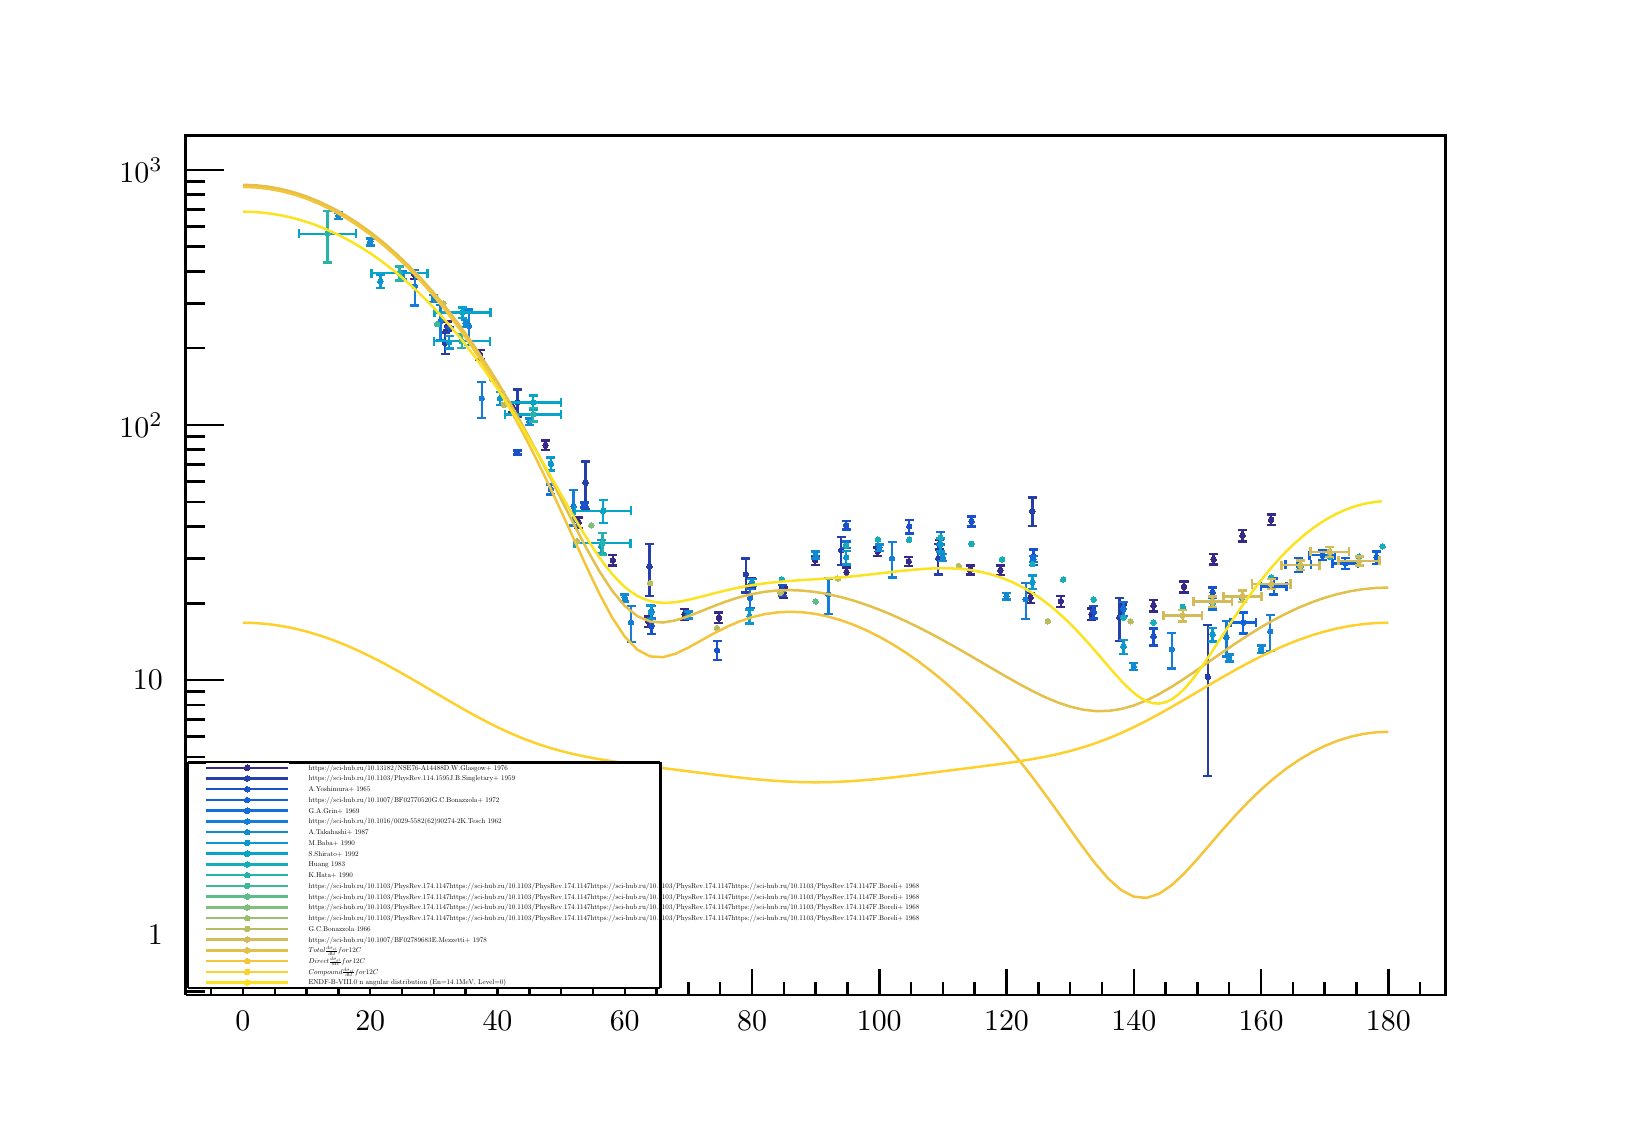
\begin{tikzpicture}
\def\CheckTikzLibraryLoaded#1{ \ifcsname tikz@library@#1@loaded\endcsname \else \PackageWarning{tikz}{usetikzlibrary{#1} is missing in the preamble.} \fi }
\CheckTikzLibraryLoaded{patterns}
\CheckTikzLibraryLoaded{plotmarks}
\pgfdeclareplotmark{cross} {
\pgfpathmoveto{\pgfpoint{-0.3\pgfplotmarksize}{\pgfplotmarksize}}
\pgfpathlineto{\pgfpoint{+0.3\pgfplotmarksize}{\pgfplotmarksize}}
\pgfpathlineto{\pgfpoint{+0.3\pgfplotmarksize}{0.3\pgfplotmarksize}}
\pgfpathlineto{\pgfpoint{+1\pgfplotmarksize}{0.3\pgfplotmarksize}}
\pgfpathlineto{\pgfpoint{+1\pgfplotmarksize}{-0.3\pgfplotmarksize}}
\pgfpathlineto{\pgfpoint{+0.3\pgfplotmarksize}{-0.3\pgfplotmarksize}}
\pgfpathlineto{\pgfpoint{+0.3\pgfplotmarksize}{-1.\pgfplotmarksize}}
\pgfpathlineto{\pgfpoint{-0.3\pgfplotmarksize}{-1.\pgfplotmarksize}}
\pgfpathlineto{\pgfpoint{-0.3\pgfplotmarksize}{-0.3\pgfplotmarksize}}
\pgfpathlineto{\pgfpoint{-1.\pgfplotmarksize}{-0.3\pgfplotmarksize}}
\pgfpathlineto{\pgfpoint{-1.\pgfplotmarksize}{0.3\pgfplotmarksize}}
\pgfpathlineto{\pgfpoint{-0.3\pgfplotmarksize}{0.3\pgfplotmarksize}}
\pgfpathclose
\pgfusepathqstroke
}
\pgfdeclareplotmark{cross*} {
\pgfpathmoveto{\pgfpoint{-0.3\pgfplotmarksize}{\pgfplotmarksize}}
\pgfpathlineto{\pgfpoint{+0.3\pgfplotmarksize}{\pgfplotmarksize}}
\pgfpathlineto{\pgfpoint{+0.3\pgfplotmarksize}{0.3\pgfplotmarksize}}
\pgfpathlineto{\pgfpoint{+1\pgfplotmarksize}{0.3\pgfplotmarksize}}
\pgfpathlineto{\pgfpoint{+1\pgfplotmarksize}{-0.3\pgfplotmarksize}}
\pgfpathlineto{\pgfpoint{+0.3\pgfplotmarksize}{-0.3\pgfplotmarksize}}
\pgfpathlineto{\pgfpoint{+0.3\pgfplotmarksize}{-1.\pgfplotmarksize}}
\pgfpathlineto{\pgfpoint{-0.3\pgfplotmarksize}{-1.\pgfplotmarksize}}
\pgfpathlineto{\pgfpoint{-0.3\pgfplotmarksize}{-0.3\pgfplotmarksize}}
\pgfpathlineto{\pgfpoint{-1.\pgfplotmarksize}{-0.3\pgfplotmarksize}}
\pgfpathlineto{\pgfpoint{-1.\pgfplotmarksize}{0.3\pgfplotmarksize}}
\pgfpathlineto{\pgfpoint{-0.3\pgfplotmarksize}{0.3\pgfplotmarksize}}
\pgfpathclose
\pgfusepathqfillstroke
}
\pgfdeclareplotmark{newstar} {
\pgfpathmoveto{\pgfqpoint{0pt}{\pgfplotmarksize}}
\pgfpathlineto{\pgfqpointpolar{44}{0.5\pgfplotmarksize}}
\pgfpathlineto{\pgfqpointpolar{18}{\pgfplotmarksize}}
\pgfpathlineto{\pgfqpointpolar{-20}{0.5\pgfplotmarksize}}
\pgfpathlineto{\pgfqpointpolar{-54}{\pgfplotmarksize}}
\pgfpathlineto{\pgfqpointpolar{-90}{0.5\pgfplotmarksize}}
\pgfpathlineto{\pgfqpointpolar{234}{\pgfplotmarksize}}
\pgfpathlineto{\pgfqpointpolar{198}{0.5\pgfplotmarksize}}
\pgfpathlineto{\pgfqpointpolar{162}{\pgfplotmarksize}}
\pgfpathlineto{\pgfqpointpolar{134}{0.5\pgfplotmarksize}}
\pgfpathclose
\pgfusepathqstroke
}
\pgfdeclareplotmark{newstar*} {
\pgfpathmoveto{\pgfqpoint{0pt}{\pgfplotmarksize}}
\pgfpathlineto{\pgfqpointpolar{44}{0.5\pgfplotmarksize}}
\pgfpathlineto{\pgfqpointpolar{18}{\pgfplotmarksize}}
\pgfpathlineto{\pgfqpointpolar{-20}{0.5\pgfplotmarksize}}
\pgfpathlineto{\pgfqpointpolar{-54}{\pgfplotmarksize}}
\pgfpathlineto{\pgfqpointpolar{-90}{0.5\pgfplotmarksize}}
\pgfpathlineto{\pgfqpointpolar{234}{\pgfplotmarksize}}
\pgfpathlineto{\pgfqpointpolar{198}{0.5\pgfplotmarksize}}
\pgfpathlineto{\pgfqpointpolar{162}{\pgfplotmarksize}}
\pgfpathlineto{\pgfqpointpolar{134}{0.5\pgfplotmarksize}}
\pgfpathclose
\pgfusepathqfillstroke
}
\definecolor{c}{rgb}{1,1,1};
\draw [color=c, fill=c] (0,0) rectangle (20,13.639);
\draw [color=c, fill=c] (2,1.3639) rectangle (18,12.2751);
\definecolor{c}{rgb}{0,0,0};
\draw [c,line width=0.9] (2,1.3639) -- (2,12.2751) -- (18,12.2751) -- (18,1.3639) -- (2,1.3639);
\draw [c,line width=0.9] (2,1.3639) -- (18,1.3639);
\draw [c,line width=0.9] (2.72727,1.69123) -- (2.72727,1.3639);
\draw [c,line width=0.9] (3.13131,1.52756) -- (3.13131,1.3639);
\draw [c,line width=0.9] (3.53535,1.52756) -- (3.53535,1.3639);
\draw [c,line width=0.9] (3.93939,1.52756) -- (3.93939,1.3639);
\draw [c,line width=0.9] (4.34343,1.69123) -- (4.34343,1.3639);
\draw [c,line width=0.9] (4.74747,1.52756) -- (4.74747,1.3639);
\draw [c,line width=0.9] (5.15152,1.52756) -- (5.15152,1.3639);
\draw [c,line width=0.9] (5.55556,1.52756) -- (5.55556,1.3639);
\draw [c,line width=0.9] (5.9596,1.69123) -- (5.9596,1.3639);
\draw [c,line width=0.9] (6.36364,1.52756) -- (6.36364,1.3639);
\draw [c,line width=0.9] (6.76768,1.52756) -- (6.76768,1.3639);
\draw [c,line width=0.9] (7.17172,1.52756) -- (7.17172,1.3639);
\draw [c,line width=0.9] (7.57576,1.69123) -- (7.57576,1.3639);
\draw [c,line width=0.9] (7.9798,1.52756) -- (7.9798,1.3639);
\draw [c,line width=0.9] (8.38384,1.52756) -- (8.38384,1.3639);
\draw [c,line width=0.9] (8.78788,1.52756) -- (8.78788,1.3639);
\draw [c,line width=0.9] (9.19192,1.69123) -- (9.19192,1.3639);
\draw [c,line width=0.9] (9.59596,1.52756) -- (9.59596,1.3639);
\draw [c,line width=0.9] (10,1.52756) -- (10,1.3639);
\draw [c,line width=0.9] (10.404,1.52756) -- (10.404,1.3639);
\draw [c,line width=0.9] (10.8081,1.69123) -- (10.8081,1.3639);
\draw [c,line width=0.9] (11.2121,1.52756) -- (11.2121,1.3639);
\draw [c,line width=0.9] (11.6162,1.52756) -- (11.6162,1.3639);
\draw [c,line width=0.9] (12.0202,1.52756) -- (12.0202,1.3639);
\draw [c,line width=0.9] (12.4242,1.69123) -- (12.4242,1.3639);
\draw [c,line width=0.9] (12.8283,1.52756) -- (12.8283,1.3639);
\draw [c,line width=0.9] (13.2323,1.52756) -- (13.2323,1.3639);
\draw [c,line width=0.9] (13.6364,1.52756) -- (13.6364,1.3639);
\draw [c,line width=0.9] (14.0404,1.69123) -- (14.0404,1.3639);
\draw [c,line width=0.9] (14.4444,1.52756) -- (14.4444,1.3639);
\draw [c,line width=0.9] (14.8485,1.52756) -- (14.8485,1.3639);
\draw [c,line width=0.9] (15.2525,1.52756) -- (15.2525,1.3639);
\draw [c,line width=0.9] (15.6566,1.69123) -- (15.6566,1.3639);
\draw [c,line width=0.9] (16.0606,1.52756) -- (16.0606,1.3639);
\draw [c,line width=0.9] (16.4646,1.52756) -- (16.4646,1.3639);
\draw [c,line width=0.9] (16.8687,1.52756) -- (16.8687,1.3639);
\draw [c,line width=0.9] (17.2727,1.69123) -- (17.2727,1.3639);
\draw [c,line width=0.9] (2.72727,1.69123) -- (2.72727,1.3639);
\draw [c,line width=0.9] (2.32323,1.52756) -- (2.32323,1.3639);
\draw [c,line width=0.9] (17.2727,1.69123) -- (17.2727,1.3639);
\draw [c,line width=0.9] (17.6768,1.52756) -- (17.6768,1.3639);
\draw [anchor=base] (2.72727,0.913811) node[scale=1.08185, color=c, rotate=0]{0};
\draw [anchor=base] (4.34343,0.913811) node[scale=1.08185, color=c, rotate=0]{20};
\draw [anchor=base] (5.9596,0.913811) node[scale=1.08185, color=c, rotate=0]{40};
\draw [anchor=base] (7.57576,0.913811) node[scale=1.08185, color=c, rotate=0]{60};
\draw [anchor=base] (9.19192,0.913811) node[scale=1.08185, color=c, rotate=0]{80};
\draw [anchor=base] (10.8081,0.913811) node[scale=1.08185, color=c, rotate=0]{100};
\draw [anchor=base] (12.4242,0.913811) node[scale=1.08185, color=c, rotate=0]{120};
\draw [anchor=base] (14.0404,0.913811) node[scale=1.08185, color=c, rotate=0]{140};
\draw [anchor=base] (15.6566,0.913811) node[scale=1.08185, color=c, rotate=0]{160};
\draw [anchor=base] (17.2727,0.913811) node[scale=1.08185, color=c, rotate=0]{180};
\draw [c,line width=0.9] (2,1.3639) -- (2,12.2751);
\draw [c,line width=0.9] (2.24,1.40279) -- (2,1.40279);
\draw [c,line width=0.9] (2.24,1.61965) -- (2,1.61965);
\draw [c,line width=0.9] (2.24,1.8075) -- (2,1.8075);
\draw [c,line width=0.9] (2.24,1.9732) -- (2,1.9732);
\draw [c,line width=0.9] (2.48,2.12143) -- (2,2.12143);
\draw [anchor= east] (1.844,2.12143) node[scale=1.08185, color=c, rotate=0]{1};
\draw [c,line width=0.9] (2.24,3.09657) -- (2,3.09657);
\draw [c,line width=0.9] (2.24,3.66698) -- (2,3.66698);
\draw [c,line width=0.9] (2.24,4.0717) -- (2,4.0717);
\draw [c,line width=0.9] (2.24,4.38563) -- (2,4.38563);
\draw [c,line width=0.9] (2.24,4.64212) -- (2,4.64212);
\draw [c,line width=0.9] (2.24,4.85898) -- (2,4.85898);
\draw [c,line width=0.9] (2.24,5.04684) -- (2,5.04684);
\draw [c,line width=0.9] (2.24,5.21254) -- (2,5.21254);
\draw [c,line width=0.9] (2.48,5.36076) -- (2,5.36076);
\draw [anchor= east] (1.844,5.36076) node[scale=1.08185, color=c, rotate=0]{10};
\draw [c,line width=0.9] (2.24,6.3359) -- (2,6.3359);
\draw [c,line width=0.9] (2.24,6.90632) -- (2,6.90632);
\draw [c,line width=0.9] (2.24,7.31104) -- (2,7.31104);
\draw [c,line width=0.9] (2.24,7.62496) -- (2,7.62496);
\draw [c,line width=0.9] (2.24,7.88146) -- (2,7.88146);
\draw [c,line width=0.9] (2.24,8.09832) -- (2,8.09832);
\draw [c,line width=0.9] (2.24,8.28618) -- (2,8.28618);
\draw [c,line width=0.9] (2.24,8.45188) -- (2,8.45188);
\draw [c,line width=0.9] (2.48,8.6001) -- (2,8.6001);
\draw [anchor= east] (1.844,8.6001) node[scale=1.08185, color=c, rotate=0]{$10^{2}$};
\draw [c,line width=0.9] (2.24,9.57524) -- (2,9.57524);
\draw [c,line width=0.9] (2.24,10.1457) -- (2,10.1457);
\draw [c,line width=0.9] (2.24,10.5504) -- (2,10.5504);
\draw [c,line width=0.9] (2.24,10.8643) -- (2,10.8643);
\draw [c,line width=0.9] (2.24,11.1208) -- (2,11.1208);
\draw [c,line width=0.9] (2.24,11.3377) -- (2,11.3377);
\draw [c,line width=0.9] (2.24,11.5255) -- (2,11.5255);
\draw [c,line width=0.9] (2.24,11.6912) -- (2,11.6912);
\draw [c,line width=0.9] (2.48,11.8394) -- (2,11.8394);
\draw [anchor= east] (1.844,11.8394) node[scale=1.08185, color=c, rotate=0]{$10^{3}$};
\definecolor{c}{rgb}{0.2082,0.1664,0.5293};
\draw [c,line width=0.9] (4.90182,10.5103) -- (4.90182,10.5668);
\draw [c,line width=0.9] (4.84451,10.5668) -- (4.95913,10.5668);
\draw [c,line width=0.9] (4.90182,10.5103) -- (4.90182,10.4513);
\draw [c,line width=0.9] (4.84451,10.4513) -- (4.95913,10.4513);
\draw [c,line width=0.9] (5.3204,9.85718) -- (5.3204,9.91465);
\draw [c,line width=0.9] (5.2631,9.91465) -- (5.37771,9.91465);
\draw [c,line width=0.9] (5.3204,9.85718) -- (5.3204,9.79726);
\draw [c,line width=0.9] (5.2631,9.79726) -- (5.37771,9.79726);
\draw [c,line width=0.9] (5.73737,9.49454) -- (5.73737,9.55305);
\draw [c,line width=0.9] (5.68007,9.55305) -- (5.79468,9.55305);
\draw [c,line width=0.9] (5.73737,9.49454) -- (5.73737,9.43349);
\draw [c,line width=0.9] (5.68007,9.43349) -- (5.79468,9.43349);
\draw [c,line width=0.9] (6.15434,8.81905) -- (6.15434,8.87685);
\draw [c,line width=0.9] (6.09703,8.87685) -- (6.21165,8.87685);
\draw [c,line width=0.9] (6.15434,8.81905) -- (6.15434,8.75878);
\draw [c,line width=0.9] (6.09703,8.75878) -- (6.21165,8.75878);
\draw [c,line width=0.9] (6.56969,8.34237) -- (6.56969,8.40127);
\draw [c,line width=0.9] (6.51238,8.40127) -- (6.627,8.40127);
\draw [c,line width=0.9] (6.56969,8.34237) -- (6.56969,8.28089);
\draw [c,line width=0.9] (6.51238,8.28089) -- (6.627,8.28089);
\draw [c,line width=0.9] (6.9907,7.35977) -- (6.9907,7.42224);
\draw [c,line width=0.9] (6.9334,7.42224) -- (7.04801,7.42224);
\draw [c,line width=0.9] (6.9907,7.35977) -- (6.9907,7.29441);
\draw [c,line width=0.9] (6.9334,7.29441) -- (7.04801,7.29441);
\draw [c,line width=0.9] (7.42464,6.88172) -- (7.42464,6.94699);
\draw [c,line width=0.9] (7.36733,6.94699) -- (7.48195,6.94699);
\draw [c,line width=0.9] (7.42464,6.88172) -- (7.42464,6.81327);
\draw [c,line width=0.9] (7.36733,6.81327) -- (7.48195,6.81327);
\draw [c,line width=0.9] (7.87797,6.10146) -- (7.87797,6.168);
\draw [c,line width=0.9] (7.82067,6.168) -- (7.93528,6.168);
\draw [c,line width=0.9] (7.87797,6.10146) -- (7.87797,6.03161);
\draw [c,line width=0.9] (7.82067,6.03161) -- (7.93528,6.03161);
\draw [c,line width=0.9] (8.33697,6.19547) -- (8.33697,6.26152);
\draw [c,line width=0.9] (8.27966,6.26152) -- (8.39427,6.26152);
\draw [c,line width=0.9] (8.33697,6.19547) -- (8.33697,6.12617);
\draw [c,line width=0.9] (8.27966,6.12617) -- (8.39427,6.12617);
\draw [c,line width=0.9] (8.77252,6.15286) -- (8.77252,6.2186);
\draw [c,line width=0.9] (8.71521,6.2186) -- (8.82983,6.2186);
\draw [c,line width=0.9] (8.77252,6.15286) -- (8.77252,6.0839);
\draw [c,line width=0.9] (8.71521,6.0839) -- (8.82983,6.0839);
\draw [c,line width=0.9] (9.18787,6.58946) -- (9.18787,6.6532);
\draw [c,line width=0.9] (9.13056,6.6532) -- (9.24518,6.6532);
\draw [c,line width=0.9] (9.18787,6.58946) -- (9.18787,6.5227);
\draw [c,line width=0.9] (9.13056,6.5227) -- (9.24518,6.5227);
\draw [c,line width=0.9] (9.59272,6.47062) -- (9.59272,6.53374);
\draw [c,line width=0.9] (9.53541,6.53374) -- (9.65003,6.53374);
\draw [c,line width=0.9] (9.59272,6.47062) -- (9.59272,6.40454);
\draw [c,line width=0.9] (9.53541,6.40454) -- (9.65003,6.40454);
\draw [c,line width=0.9] (9.99353,6.87981) -- (9.99353,6.93602);
\draw [c,line width=0.9] (9.93622,6.93602) -- (10.0508,6.93602);
\draw [c,line width=0.9] (9.99353,6.87981) -- (9.99353,6.82127);
\draw [c,line width=0.9] (9.93622,6.82127) -- (10.0508,6.82127);
\draw [c,line width=0.9] (10.3919,6.73127) -- (10.3919,6.79054);
\draw [c,line width=0.9] (10.3346,6.79054) -- (10.4492,6.79054);
\draw [c,line width=0.9] (10.3919,6.73127) -- (10.3919,6.66938);
\draw [c,line width=0.9] (10.3346,6.66938) -- (10.4492,6.66938);
\draw [c,line width=0.9] (10.7887,6.99139) -- (10.7887,7.04466);
\draw [c,line width=0.9] (10.7314,7.04466) -- (10.846,7.04466);
\draw [c,line width=0.9] (10.7887,6.99139) -- (10.7887,6.93602);
\draw [c,line width=0.9] (10.7314,6.93602) -- (10.846,6.93602);
\draw [c,line width=0.9] (11.183,6.86685) -- (11.183,6.92125);
\draw [c,line width=0.9] (11.1257,6.92125) -- (11.2403,6.92125);
\draw [c,line width=0.9] (11.183,6.86685) -- (11.183,6.81026);
\draw [c,line width=0.9] (11.1257,6.81026) -- (11.2403,6.81026);
\draw [c,line width=0.9] (11.5725,7.07909) -- (11.5725,7.13758);
\draw [c,line width=0.9] (11.5152,7.13758) -- (11.6298,7.13758);
\draw [c,line width=0.9] (11.5725,7.07909) -- (11.5725,7.01806);
\draw [c,line width=0.9] (11.5152,7.01806) -- (11.6298,7.01806);
\draw [c,line width=0.9] (11.9612,6.76122) -- (11.9612,6.81627);
\draw [c,line width=0.9] (11.9039,6.81627) -- (12.0185,6.81627);
\draw [c,line width=0.9] (11.9612,6.76122) -- (11.9612,6.70392);
\draw [c,line width=0.9] (11.9039,6.70392) -- (12.0185,6.70392);
\draw [c,line width=0.9] (12.3458,6.75549) -- (12.3458,6.81627);
\draw [c,line width=0.9] (12.2885,6.81627) -- (12.4032,6.81627);
\draw [c,line width=0.9] (12.3458,6.75549) -- (12.3458,6.69195);
\draw [c,line width=0.9] (12.2885,6.69195) -- (12.4032,6.69195);
\draw [c,line width=0.9] (12.7297,6.40588) -- (12.7297,6.46678);
\draw [c,line width=0.9] (12.6724,6.46678) -- (12.787,6.46678);
\draw [c,line width=0.9] (12.7297,6.40588) -- (12.7297,6.34222);
\draw [c,line width=0.9] (12.6724,6.34222) -- (12.787,6.34222);
\draw [c,line width=0.9] (13.1143,6.35962) -- (13.1143,6.42648);
\draw [c,line width=0.9] (13.057,6.42648) -- (13.1716,6.42648);
\draw [c,line width=0.9] (13.1143,6.35962) -- (13.1143,6.28942);
\draw [c,line width=0.9] (13.057,6.28942) -- (13.1716,6.28942);
\draw [c,line width=0.9] (13.5038,6.19935) -- (13.5038,6.26891);
\draw [c,line width=0.9] (13.4465,6.26891) -- (13.5611,6.26891);
\draw [c,line width=0.9] (13.5038,6.19935) -- (13.5038,6.12617);
\draw [c,line width=0.9] (13.4465,6.12617) -- (13.5611,6.12617);
\draw [c,line width=0.9] (13.8966,6.24661) -- (13.8966,6.3182);
\draw [c,line width=0.9] (13.8392,6.3182) -- (13.9539,6.3182);
\draw [c,line width=0.9] (13.8966,6.24661) -- (13.8966,6.17117);
\draw [c,line width=0.9] (13.8392,6.17117) -- (13.9539,6.17117);
\draw [c,line width=0.9] (14.2909,6.3046) -- (14.2909,6.37475);
\draw [c,line width=0.9] (14.2336,6.37475) -- (14.3482,6.37475);
\draw [c,line width=0.9] (14.2909,6.3046) -- (14.2909,6.23078);
\draw [c,line width=0.9] (14.2336,6.23078) -- (14.3482,6.23078);
\draw [c,line width=0.9] (14.678,6.5447) -- (14.678,6.61507);
\draw [c,line width=0.9] (14.6207,6.61507) -- (14.7353,6.61507);
\draw [c,line width=0.9] (14.678,6.5447) -- (14.678,6.47062);
\draw [c,line width=0.9] (14.6207,6.47062) -- (14.7353,6.47062);
\draw [c,line width=0.9] (15.0545,6.89407) -- (15.0545,6.95969);
\draw [c,line width=0.9] (14.9972,6.95969) -- (15.1118,6.95969);
\draw [c,line width=0.9] (15.0545,6.89407) -- (15.0545,6.82524);
\draw [c,line width=0.9] (14.9972,6.82524) -- (15.1118,6.82524);
\draw [c,line width=0.9] (15.4222,7.19373) -- (15.4222,7.26565);
\draw [c,line width=0.9] (15.3649,7.26565) -- (15.4795,7.26565);
\draw [c,line width=0.9] (15.4222,7.19373) -- (15.4222,7.11795);
\draw [c,line width=0.9] (15.3649,7.11795) -- (15.4795,7.11795);
\draw [c,line width=0.9] (15.7842,7.39666) -- (15.7842,7.46291);
\draw [c,line width=0.9] (15.7269,7.46291) -- (15.8415,7.46291);
\draw [c,line width=0.9] (15.7842,7.39666) -- (15.7842,7.32712);
\draw [c,line width=0.9] (15.7269,7.32712) -- (15.8415,7.32712);
\foreach \P in {(4.90182,10.5103), (5.3204,9.85718), (5.73737,9.49454), (6.15434,8.81905), (6.56969,8.34237), (6.9907,7.35977), (7.42464,6.88172), (7.87797,6.10146), (8.33697,6.19547), (8.77252,6.15286), (9.18787,6.58946), (9.59272,6.47062),
 (9.99353,6.87981), (10.3919,6.73127), (10.7887,6.99139), (11.183,6.86685), (11.5725,7.07909), (11.9612,6.76122), (12.3458,6.75549), (12.7297,6.40588), (13.1143,6.35962), (13.5038,6.19935), (13.8966,6.24661), (14.2909,6.3046), (14.678,6.5447),
 (15.0545,6.89407), (15.4222,7.19373), (15.7842,7.39666)}{\draw[mark options={color=c,fill=c},mark size=2.402402pt, line width=0.000000pt, mark=*,mark size=1pt] plot coordinates {\P};}
\definecolor{c}{rgb}{0.150523,0.241303,0.660565};
\draw [c,line width=0.9] (5.29602,9.64388) -- (5.29602,9.77186);
\draw [c,line width=0.9] (5.23871,9.77186) -- (5.35333,9.77186);
\draw [c,line width=0.9] (5.29602,9.64388) -- (5.29602,9.50308);
\draw [c,line width=0.9] (5.23871,9.50308) -- (5.35333,9.50308);
\draw [c,line width=0.9] (6.21119,8.89133) -- (6.21119,9.05322);
\draw [c,line width=0.9] (6.15389,9.05322) -- (6.2685,9.05322);
\draw [c,line width=0.9] (6.21119,8.89133) -- (6.21119,8.70837);
\draw [c,line width=0.9] (6.15389,8.70837) -- (6.2685,8.70837);
\draw [c,line width=0.9] (7.07821,7.86495) -- (7.07821,8.13404);
\draw [c,line width=0.9] (7.02091,8.13404) -- (7.13552,8.13404);
\draw [c,line width=0.9] (7.07821,7.86495) -- (7.07821,7.53191);
\draw [c,line width=0.9] (7.02091,7.53191) -- (7.13552,7.53191);
\draw [c,line width=0.9] (7.89058,6.79917) -- (7.89058,7.09065);
\draw [c,line width=0.9] (7.83328,7.09065) -- (7.94789,7.09065);
\draw [c,line width=0.9] (7.89058,6.79917) -- (7.89058,6.43108);
\draw [c,line width=0.9] (7.83328,6.43108) -- (7.94789,6.43108);
\draw [c,line width=0.9] (9.11491,6.705) -- (9.11491,6.90632);
\draw [c,line width=0.9] (9.0576,6.90632) -- (9.17222,6.90632);
\draw [c,line width=0.9] (9.11491,6.705) -- (9.11491,6.46999);
\draw [c,line width=0.9] (9.0576,6.46999) -- (9.17222,6.46999);
\draw [c,line width=0.9] (10.3243,7.01024) -- (10.3243,7.17449);
\draw [c,line width=0.9] (10.267,7.17449) -- (10.3817,7.17449);
\draw [c,line width=0.9] (10.3243,7.01024) -- (10.3243,6.82425);
\draw [c,line width=0.9] (10.267,6.82425) -- (10.3817,6.82425);
\draw [c,line width=0.9] (11.5571,6.90632) -- (11.5571,7.08653);
\draw [c,line width=0.9] (11.4997,7.08653) -- (11.6144,7.08653);
\draw [c,line width=0.9] (11.5571,6.90632) -- (11.5571,6.69958);
\draw [c,line width=0.9] (11.4997,6.69958) -- (11.6144,6.69958);
\draw [c,line width=0.9] (12.752,7.50766) -- (12.752,7.67743);
\draw [c,line width=0.9] (12.6947,7.67743) -- (12.8093,7.67743);
\draw [c,line width=0.9] (12.752,7.50766) -- (12.752,7.31455);
\draw [c,line width=0.9] (12.6947,7.31455) -- (12.8093,7.31455);
\draw [c,line width=0.9] (13.8571,6.15606) -- (13.8571,6.40454);
\draw [c,line width=0.9] (13.7998,6.40454) -- (13.9144,6.40454);
\draw [c,line width=0.9] (13.8571,6.15606) -- (13.8571,5.85408);
\draw [c,line width=0.9] (13.7998,5.85408) -- (13.9144,5.85408);
\draw [c,line width=0.9] (14.9812,5.40235) -- (14.9812,6.05671);
\draw [c,line width=0.9] (14.9239,6.05671) -- (15.0385,6.05671);
\draw [c,line width=0.9] (14.9812,5.40235) -- (14.9812,4.14034);
\draw [c,line width=0.9] (14.9239,4.14034) -- (15.0385,4.14034);
\foreach \P in {(5.29602,9.64388), (6.21119,8.89133), (7.07821,7.86495), (7.89058,6.79917), (9.11491,6.705), (10.3243,7.01024), (11.5571,6.90632), (12.752,7.50766), (13.8571,6.15606), (14.9812,5.40235)}{\draw[mark options={color=c,fill=c},mark
 size=2.402402pt, line width=0.000000pt, mark=*,mark size=1pt] plot coordinates {\P};}
\definecolor{c}{rgb}{0.0928452,0.316206,0.791829};
\draw [c,line width=0.9] (15.0424,6.47637) -- (15.0424,6.53923);
\draw [c,line width=0.9] (14.9851,6.53923) -- (15.0997,6.53923);
\draw [c,line width=0.9] (15.0424,6.47637) -- (15.0424,6.41056);
\draw [c,line width=0.9] (14.9851,6.41056) -- (15.0997,6.41056);
\draw [c,line width=0.9] (14.291,5.9123) -- (14.291,6.01404);
\draw [c,line width=0.9] (14.2337,6.01404) -- (14.3483,6.01404);
\draw [c,line width=0.9] (14.291,5.9123) -- (14.291,5.80262);
\draw [c,line width=0.9] (14.2337,5.80262) -- (14.3483,5.80262);
\draw [c,line width=0.9] (13.5314,6.22622) -- (13.5314,6.30317);
\draw [c,line width=0.9] (13.4741,6.30317) -- (13.5887,6.30317);
\draw [c,line width=0.9] (13.5314,6.22622) -- (13.5314,6.14483);
\draw [c,line width=0.9] (13.4741,6.14483) -- (13.5887,6.14483);
\draw [c,line width=0.9] (12.7637,6.92495) -- (12.7637,7.01849);
\draw [c,line width=0.9] (12.7064,7.01849) -- (12.821,7.01849);
\draw [c,line width=0.9] (12.7637,6.92495) -- (12.7637,6.82475);
\draw [c,line width=0.9] (12.7064,6.82475) -- (12.821,6.82475);
\draw [c,line width=0.9] (11.9798,7.37632) -- (11.9798,7.43968);
\draw [c,line width=0.9] (11.9225,7.43968) -- (12.0371,7.43968);
\draw [c,line width=0.9] (11.9798,7.37632) -- (11.9798,7.30998);
\draw [c,line width=0.9] (11.9225,7.30998) -- (12.0371,7.30998);
\draw [c,line width=0.9] (11.1881,7.31104) -- (11.1881,7.395);
\draw [c,line width=0.9] (11.1308,7.395) -- (11.2454,7.395);
\draw [c,line width=0.9] (11.1881,7.31104) -- (11.1881,7.22174);
\draw [c,line width=0.9] (11.1308,7.22174) -- (11.2454,7.22174);
\draw [c,line width=0.9] (10.388,7.32851) -- (10.388,7.38068);
\draw [c,line width=0.9] (10.3307,7.38068) -- (10.4453,7.38068);
\draw [c,line width=0.9] (10.388,7.32851) -- (10.388,7.27434);
\draw [c,line width=0.9] (10.3307,7.27434) -- (10.4453,7.27434);
\draw [c,line width=0.9] (9.57993,6.5016) -- (9.57993,6.56935);
\draw [c,line width=0.9] (9.52263,6.56935) -- (9.63724,6.56935);
\draw [c,line width=0.9] (9.57993,6.5016) -- (9.57993,6.43043);
\draw [c,line width=0.9] (9.52263,6.43043) -- (9.63724,6.43043);
\draw [c,line width=0.9] (8.74765,5.74064) -- (8.74765,5.85803);
\draw [c,line width=0.9] (8.69034,5.85803) -- (8.80495,5.85803);
\draw [c,line width=0.9] (8.74765,5.74064) -- (8.74765,5.61256);
\draw [c,line width=0.9] (8.69034,5.61256) -- (8.80495,5.61256);
\draw [c,line width=0.9] (7.9153,6.04811) -- (7.9153,6.1416);
\draw [c,line width=0.9] (7.85799,6.1416) -- (7.97261,6.1416);
\draw [c,line width=0.9] (7.9153,6.04811) -- (7.9153,5.94796);
\draw [c,line width=0.9] (7.85799,5.94796) -- (7.97261,5.94796);
\draw [c,line width=0.9] (7.06673,7.58501) -- (7.06673,7.61536);
\draw [c,line width=0.9] (7.00943,7.61536) -- (7.12404,7.61536);
\draw [c,line width=0.9] (7.06673,7.58501) -- (7.06673,7.55399);
\draw [c,line width=0.9] (7.00943,7.55399) -- (7.12404,7.55399);
\draw [c,line width=0.9] (6.20984,8.25056) -- (6.20984,8.2731);
\draw [c,line width=0.9] (6.15253,8.2731) -- (6.26714,8.2731);
\draw [c,line width=0.9] (6.20984,8.25056) -- (6.20984,8.22765);
\draw [c,line width=0.9] (6.15253,8.22765) -- (6.26714,8.22765);
\draw [c,line width=0.9] (5.34569,9.83758) -- (5.34569,9.84102);
\draw [c,line width=0.9] (5.28838,9.84102) -- (5.403,9.84102);
\draw [c,line width=0.9] (5.34569,9.83758) -- (5.34569,9.83413);
\draw [c,line width=0.9] (5.28838,9.83413) -- (5.403,9.83413);
\foreach \P in {(15.0424,6.47637), (14.291,5.9123), (13.5314,6.22622), (12.7637,6.92495), (11.9798,7.37632), (11.1881,7.31104), (10.388,7.32851), (9.57993,6.5016), (8.74765,5.74064), (7.9153,6.04811), (7.06673,7.58501), (6.20984,8.25056),
 (5.34569,9.83758)}{\draw[mark options={color=c,fill=c},mark size=2.402402pt, line width=0.000000pt, mark=*,mark size=1pt] plot coordinates {\P};}
\definecolor{c}{rgb}{0.0621375,0.382431,0.863728};
\draw [c,line width=0.9] (15.4303,6.09062) -- (15.2685,6.09062);
\draw [c,line width=0.9] (15.2685,6.03331) -- (15.2685,6.14792);
\draw [c,line width=0.9] (15.4303,6.09062) -- (15.5921,6.09062);
\draw [c,line width=0.9] (15.5921,6.03331) -- (15.5921,6.14792);
\draw [c,line width=0.9] (15.4303,6.09062) -- (15.4303,6.2186);
\draw [c,line width=0.9] (15.373,6.2186) -- (15.4876,6.2186);
\draw [c,line width=0.9] (15.4303,6.09062) -- (15.4303,5.94982);
\draw [c,line width=0.9] (15.373,5.94982) -- (15.4876,5.94982);
\draw [c,line width=0.9] (15.8182,6.55075) -- (15.6563,6.55075);
\draw [c,line width=0.9] (15.6563,6.49345) -- (15.6563,6.60806);
\draw [c,line width=0.9] (15.8182,6.55075) -- (15.98,6.55075);
\draw [c,line width=0.9] (15.98,6.49345) -- (15.98,6.60806);
\draw [c,line width=0.9] (15.8182,6.55075) -- (15.8182,6.64982);
\draw [c,line width=0.9] (15.7609,6.64982) -- (15.8755,6.64982);
\draw [c,line width=0.9] (15.8182,6.55075) -- (15.8182,6.44417);
\draw [c,line width=0.9] (15.7609,6.44417) -- (15.8755,6.44417);
\draw [c,line width=0.9] (16.1309,6.82425) -- (15.9689,6.82425);
\draw [c,line width=0.9] (15.9689,6.76694) -- (15.9689,6.88156);
\draw [c,line width=0.9] (16.1309,6.82425) -- (16.2929,6.82425);
\draw [c,line width=0.9] (16.2929,6.76694) -- (16.2929,6.88156);
\draw [c,line width=0.9] (16.1309,6.82425) -- (16.1309,6.911);
\draw [c,line width=0.9] (16.0736,6.911) -- (16.1882,6.911);
\draw [c,line width=0.9] (16.1309,6.82425) -- (16.1309,6.7318);
\draw [c,line width=0.9] (16.0736,6.7318) -- (16.1882,6.7318);
\draw [c,line width=0.9] (16.4363,6.9479) -- (16.274,6.9479);
\draw [c,line width=0.9] (16.274,6.8906) -- (16.274,7.00521);
\draw [c,line width=0.9] (16.4363,6.9479) -- (16.5987,6.9479);
\draw [c,line width=0.9] (16.5987,6.8906) -- (16.5987,7.00521);
\draw [c,line width=0.9] (16.4363,6.9479) -- (16.4363,7.01024);
\draw [c,line width=0.9] (16.379,7.01024) -- (16.4936,7.01024);
\draw [c,line width=0.9] (16.4363,6.9479) -- (16.4363,6.88267);
\draw [c,line width=0.9] (16.379,6.88267) -- (16.4936,6.88267);
\draw [c,line width=0.9] (16.7248,6.844) -- (16.5614,6.844);
\draw [c,line width=0.9] (16.5614,6.78669) -- (16.5614,6.9013);
\draw [c,line width=0.9] (16.7248,6.844) -- (16.8882,6.844);
\draw [c,line width=0.9] (16.8882,6.78669) -- (16.8882,6.9013);
\draw [c,line width=0.9] (16.7248,6.844) -- (16.7248,6.911);
\draw [c,line width=0.9] (16.6675,6.911) -- (16.7821,6.911);
\draw [c,line width=0.9] (16.7248,6.844) -- (16.7248,6.77364);
\draw [c,line width=0.9] (16.6675,6.77364) -- (16.7821,6.77364);
\draw [c,line width=0.9] (17.1248,6.91753) -- (17.1248,6.99447);
\draw [c,line width=0.9] (17.0675,6.99447) -- (17.1821,6.99447);
\draw [c,line width=0.9] (17.1248,6.91753) -- (17.1248,6.83613);
\draw [c,line width=0.9] (17.0675,6.83613) -- (17.1821,6.83613);
\foreach \P in {(15.4303,6.09062), (15.8182,6.55075), (16.1309,6.82425), (16.4363,6.9479), (16.7248,6.844), (17.1248,6.91753)}{\draw[mark options={color=c,fill=c},mark size=2.402402pt, line width=0.000000pt, mark=*,mark size=1pt] plot coordinates
 {\P};}
\definecolor{c}{rgb}{0.0691875,0.436506,0.852516};
\draw [c,line width=0.9] (15.0424,6.3359) -- (15.0424,6.41122);
\draw [c,line width=0.9] (14.9851,6.41122) -- (15.0997,6.41122);
\draw [c,line width=0.9] (15.0424,6.3359) -- (15.0424,6.25632);
\draw [c,line width=0.9] (14.9851,6.25632) -- (15.0997,6.25632);
\draw [c,line width=0.9] (13.9111,6.26374) -- (13.9111,6.3499);
\draw [c,line width=0.9] (13.8538,6.3499) -- (13.9684,6.3499);
\draw [c,line width=0.9] (13.9111,6.26374) -- (13.9111,6.17196);
\draw [c,line width=0.9] (13.8538,6.17196) -- (13.9684,6.17196);
\draw [c,line width=0.9] (12.7637,6.89691) -- (12.7637,6.93418);
\draw [c,line width=0.9] (12.7064,6.93418) -- (12.821,6.93418);
\draw [c,line width=0.9] (12.7637,6.89691) -- (12.7637,6.85863);
\draw [c,line width=0.9] (12.7064,6.85863) -- (12.821,6.85863);
\draw [c,line width=0.9] (11.5919,7.16281) -- (11.5919,7.23888);
\draw [c,line width=0.9] (11.5346,7.23888) -- (11.6492,7.23888);
\draw [c,line width=0.9] (11.5919,7.16281) -- (11.5919,7.0824);
\draw [c,line width=0.9] (11.5346,7.0824) -- (11.6492,7.0824);
\draw [c,line width=0.9] (10.388,7.0824) -- (10.388,7.12318);
\draw [c,line width=0.9] (10.3307,7.12318) -- (10.4453,7.12318);
\draw [c,line width=0.9] (10.388,7.0824) -- (10.388,7.0404);
\draw [c,line width=0.9] (10.3307,7.0404) -- (10.4453,7.0404);
\draw [c,line width=0.9] (9.16767,6.40454) -- (9.16767,6.52023);
\draw [c,line width=0.9] (9.11037,6.52023) -- (9.22498,6.52023);
\draw [c,line width=0.9] (9.16767,6.40454) -- (9.16767,6.27847);
\draw [c,line width=0.9] (9.11037,6.27847) -- (9.22498,6.27847);
\draw [c,line width=0.9] (7.9153,6.22622) -- (7.9153,6.30028);
\draw [c,line width=0.9] (7.85799,6.30028) -- (7.97261,6.30028);
\draw [c,line width=0.9] (7.9153,6.22622) -- (7.9153,6.14804);
\draw [c,line width=0.9] (7.85799,6.14804) -- (7.97261,6.14804);
\draw [c,line width=0.9] (6.63854,7.7844) -- (6.63854,7.84584);
\draw [c,line width=0.9] (6.58123,7.84584) -- (6.69584,7.84584);
\draw [c,line width=0.9] (6.63854,7.7844) -- (6.63854,7.72015);
\draw [c,line width=0.9] (6.58123,7.72015) -- (6.69584,7.72015);
\foreach \P in {(15.0424,6.3359), (13.9111,6.26374), (12.7637,6.89691), (11.5919,7.16281), (10.388,7.0824), (9.16767,6.40454), (7.9153,6.22622), (6.63854,7.7844)}{\draw[mark options={color=c,fill=c},mark size=2.402402pt, line width=0.000000pt,
 mark=*,mark size=1pt] plot coordinates {\P};}
\definecolor{c}{rgb}{0.0762375,0.490581,0.841303};
\draw [c,line width=0.9] (15.773,5.97731) -- (15.773,6.18611);
\draw [c,line width=0.9] (15.7157,6.18611) -- (15.8303,6.18611);
\draw [c,line width=0.9] (15.773,5.97731) -- (15.773,5.73203);
\draw [c,line width=0.9] (15.7157,5.73203) -- (15.8303,5.73203);
\draw [c,line width=0.9] (15.2166,5.90276) -- (15.2166,6.11156);
\draw [c,line width=0.9] (15.1593,6.11156) -- (15.2739,6.11156);
\draw [c,line width=0.9] (15.2166,5.90276) -- (15.2166,5.65747);
\draw [c,line width=0.9] (15.1593,5.65747) -- (15.2739,5.65747);
\draw [c,line width=0.9] (14.5249,5.75134) -- (14.5249,5.96014);
\draw [c,line width=0.9] (14.4676,5.96014) -- (14.5822,5.96014);
\draw [c,line width=0.9] (14.5249,5.75134) -- (14.5249,5.50606);
\draw [c,line width=0.9] (14.4676,5.50606) -- (14.5822,5.50606);
\draw [c,line width=0.9] (12.6686,6.3843) -- (12.6686,6.5931);
\draw [c,line width=0.9] (12.6113,6.5931) -- (12.7259,6.5931);
\draw [c,line width=0.9] (12.6686,6.3843) -- (12.6686,6.13901);
\draw [c,line width=0.9] (12.6113,6.13901) -- (12.7259,6.13901);
\draw [c,line width=0.9] (10.9701,6.90632) -- (10.9701,7.11512);
\draw [c,line width=0.9] (10.9128,7.11512) -- (11.0274,7.11512);
\draw [c,line width=0.9] (10.9701,6.90632) -- (10.9701,6.66103);
\draw [c,line width=0.9] (10.9128,6.66103) -- (11.0274,6.66103);
\draw [c,line width=0.9] (10.1621,6.44417) -- (10.1621,6.65297);
\draw [c,line width=0.9] (10.1048,6.65297) -- (10.2194,6.65297);
\draw [c,line width=0.9] (10.1621,6.44417) -- (10.1621,6.19889);
\draw [c,line width=0.9] (10.1048,6.19889) -- (10.2194,6.19889);
\draw [c,line width=0.9] (7.65555,6.09062) -- (7.65555,6.29942);
\draw [c,line width=0.9] (7.59824,6.29942) -- (7.71285,6.29942);
\draw [c,line width=0.9] (7.65555,6.09062) -- (7.65555,5.84533);
\draw [c,line width=0.9] (7.59824,5.84533) -- (7.71285,5.84533);
\draw [c,line width=0.9] (6.92729,7.56753) -- (6.92729,7.77633);
\draw [c,line width=0.9] (6.86999,7.77633) -- (6.9846,7.77633);
\draw [c,line width=0.9] (6.92729,7.56753) -- (6.92729,7.32225);
\draw [c,line width=0.9] (6.86999,7.32225) -- (6.9846,7.32225);
\draw [c,line width=0.9] (5.76025,8.93636) -- (5.76025,9.14516);
\draw [c,line width=0.9] (5.70295,9.14516) -- (5.81756,9.14516);
\draw [c,line width=0.9] (5.76025,8.93636) -- (5.76025,8.69107);
\draw [c,line width=0.9] (5.70295,8.69107) -- (5.81756,8.69107);
\draw [c,line width=0.9] (5.59687,9.86074) -- (5.59687,10.0695);
\draw [c,line width=0.9] (5.53957,10.0695) -- (5.65418,10.0695);
\draw [c,line width=0.9] (5.59687,9.86074) -- (5.59687,9.61546);
\draw [c,line width=0.9] (5.53957,9.61546) -- (5.65418,9.61546);
\draw [c,line width=0.9] (5.23382,9.91702) -- (5.23382,10.1258);
\draw [c,line width=0.9] (5.17651,10.1258) -- (5.29113,10.1258);
\draw [c,line width=0.9] (5.23382,9.91702) -- (5.23382,9.67174);
\draw [c,line width=0.9] (5.17651,9.67174) -- (5.29113,9.67174);
\draw [c,line width=0.9] (4.90915,10.3625) -- (4.90915,10.5713);
\draw [c,line width=0.9] (4.85185,10.5713) -- (4.96646,10.5713);
\draw [c,line width=0.9] (4.90915,10.3625) -- (4.90915,10.1172);
\draw [c,line width=0.9] (4.85185,10.1172) -- (4.96646,10.1172);
\foreach \P in {(15.773,5.97731), (15.2166,5.90276), (14.5249,5.75134), (12.6686,6.3843), (10.9701,6.90632), (10.1621,6.44417), (7.65555,6.09062), (6.92729,7.56753), (5.76025,8.93636), (5.59687,9.86074), (5.23382,9.91702),
 (4.90915,10.3625)}{\draw[mark options={color=c,fill=c},mark size=2.402402pt, line width=0.000000pt, mark=*,mark size=1pt] plot coordinates {\P};}
\definecolor{c}{rgb}{0.0625875,0.542856,0.825253};
\draw [c,line width=0.9] (3.93939,11.2591) -- (3.93939,11.301);
\draw [c,line width=0.9] (3.88208,11.301) -- (3.99669,11.301);
\draw [c,line width=0.9] (3.93939,11.2591) -- (3.93939,11.216);
\draw [c,line width=0.9] (3.88208,11.216) -- (3.99669,11.216);
\draw [c,line width=0.9] (4.34344,10.9249) -- (4.34344,10.97);
\draw [c,line width=0.9] (4.28613,10.97) -- (4.40075,10.97);
\draw [c,line width=0.9] (4.34344,10.9249) -- (4.34344,10.8783);
\draw [c,line width=0.9] (4.28613,10.8783) -- (4.40075,10.8783);
\draw [c,line width=0.9] (4.74747,10.5039) -- (4.74747,10.5504);
\draw [c,line width=0.9] (4.69016,10.5504) -- (4.80477,10.5504);
\draw [c,line width=0.9] (4.74747,10.5039) -- (4.74747,10.4558);
\draw [c,line width=0.9] (4.69016,10.4558) -- (4.80477,10.4558);
\draw [c,line width=0.9] (5.15151,10.2053) -- (5.15151,10.2496);
\draw [c,line width=0.9] (5.09421,10.2496) -- (5.20882,10.2496);
\draw [c,line width=0.9] (5.15151,10.2053) -- (5.15151,10.1597);
\draw [c,line width=0.9] (5.09421,10.1597) -- (5.20882,10.1597);
\draw [c,line width=0.9] (5.55555,9.88916) -- (5.55555,9.93075);
\draw [c,line width=0.9] (5.49824,9.93075) -- (5.61286,9.93075);
\draw [c,line width=0.9] (5.55555,9.88916) -- (5.55555,9.84631);
\draw [c,line width=0.9] (5.49824,9.84631) -- (5.61286,9.84631);
\draw [c,line width=0.9] (6.36363,8.64168) -- (6.36363,8.6834);
\draw [c,line width=0.9] (6.30633,8.6834) -- (6.42094,8.6834);
\draw [c,line width=0.9] (6.36363,8.64168) -- (6.36363,8.59869);
\draw [c,line width=0.9] (6.30633,8.59869) -- (6.42094,8.59869);
\draw [c,line width=0.9] (7.57575,6.40454) -- (7.57575,6.44742);
\draw [c,line width=0.9] (7.51845,6.44742) -- (7.63306,6.44742);
\draw [c,line width=0.9] (7.57575,6.40454) -- (7.57575,6.36031);
\draw [c,line width=0.9] (7.51845,6.36031) -- (7.63306,6.36031);
\draw [c,line width=0.9] (8.38383,6.18768) -- (8.38383,6.23381);
\draw [c,line width=0.9] (8.32652,6.23381) -- (8.44114,6.23381);
\draw [c,line width=0.9] (8.38383,6.18768) -- (8.38383,6.13998);
\draw [c,line width=0.9] (8.32652,6.13998) -- (8.44114,6.13998);
\draw [c,line width=0.9] (9.19191,6.60407) -- (9.19191,6.64588);
\draw [c,line width=0.9] (9.13461,6.64588) -- (9.24922,6.64588);
\draw [c,line width=0.9] (9.19191,6.60407) -- (9.19191,6.56098);
\draw [c,line width=0.9] (9.13461,6.56098) -- (9.24922,6.56098);
\draw [c,line width=0.9] (9.99998,6.9479) -- (9.99998,6.99095);
\draw [c,line width=0.9] (9.94268,6.99095) -- (10.0573,6.99095);
\draw [c,line width=0.9] (9.99998,6.9479) -- (9.99998,6.9035);
\draw [c,line width=0.9] (9.94268,6.9035) -- (10.0573,6.9035);
\draw [c,line width=0.9] (10.8081,7.0404) -- (10.8081,7.08199);
\draw [c,line width=0.9] (10.7508,7.08199) -- (10.8654,7.08199);
\draw [c,line width=0.9] (10.8081,7.0404) -- (10.8081,6.99755);
\draw [c,line width=0.9] (10.7508,6.99755) -- (10.8654,6.99755);
\draw [c,line width=0.9] (11.6162,6.91567) -- (11.6162,6.95924);
\draw [c,line width=0.9] (11.5588,6.95924) -- (11.6735,6.95924);
\draw [c,line width=0.9] (11.6162,6.91567) -- (11.6162,6.8707);
\draw [c,line width=0.9] (11.5588,6.8707) -- (11.6735,6.8707);
\draw [c,line width=0.9] (12.4242,6.42449) -- (12.4242,6.46678);
\draw [c,line width=0.9] (12.3669,6.46678) -- (12.4815,6.46678);
\draw [c,line width=0.9] (12.4242,6.42449) -- (12.4242,6.38089);
\draw [c,line width=0.9] (12.3669,6.38089) -- (12.4815,6.38089);
\draw [c,line width=0.9] (14.0404,5.5327) -- (14.0404,5.57561);
\draw [c,line width=0.9] (13.9831,5.57561) -- (14.0977,5.57561);
\draw [c,line width=0.9] (14.0404,5.5327) -- (14.0404,5.48844);
\draw [c,line width=0.9] (13.9831,5.48844) -- (14.0977,5.48844);
\draw [c,line width=0.9] (15.2525,5.64051) -- (15.2525,5.68254);
\draw [c,line width=0.9] (15.1952,5.68254) -- (15.3098,5.68254);
\draw [c,line width=0.9] (15.2525,5.64051) -- (15.2525,5.59718);
\draw [c,line width=0.9] (15.1952,5.59718) -- (15.3098,5.59718);
\draw [c,line width=0.9] (15.6566,5.75134) -- (15.6566,5.7985);
\draw [c,line width=0.9] (15.5992,5.7985) -- (15.7139,5.7985);
\draw [c,line width=0.9] (15.6566,5.75134) -- (15.6566,5.70255);
\draw [c,line width=0.9] (15.5992,5.70255) -- (15.7139,5.70255);
\foreach \P in {(3.93939,11.2591), (4.34344,10.9249), (4.74747,10.5039), (5.15151,10.2053), (5.55555,9.88916), (6.36363,8.64168), (7.57575,6.40454), (8.38383,6.18768), (9.19191,6.60407), (9.99998,6.9479), (10.8081,7.0404), (11.6162,6.91567),
 (12.4242,6.42449), (14.0404,5.5327), (15.2525,5.64051), (15.6566,5.75134)}{\draw[mark options={color=c,fill=c},mark size=2.402402pt, line width=0.000000pt, mark=*,mark size=1pt] plot coordinates {\P};}
\definecolor{c}{rgb}{0.0420375,0.594531,0.807591};
\draw [c,line width=0.9] (4.47273,10.4246) -- (4.47273,10.5018);
\draw [c,line width=0.9] (4.41542,10.5018) -- (4.53004,10.5018);
\draw [c,line width=0.9] (4.47273,10.4246) -- (4.47273,10.3428);
\draw [c,line width=0.9] (4.41542,10.3428) -- (4.53004,10.3428);
\draw [c,line width=0.9] (5.34545,9.65176) -- (5.34545,9.72932);
\draw [c,line width=0.9] (5.28814,9.72932) -- (5.40275,9.72932);
\draw [c,line width=0.9] (5.34545,9.65176) -- (5.34545,9.56967);
\draw [c,line width=0.9] (5.28814,9.56967) -- (5.40275,9.56967);
\draw [c,line width=0.9] (5.99191,8.93835) -- (5.99191,9.01603);
\draw [c,line width=0.9] (5.93461,9.01603) -- (6.04922,9.01603);
\draw [c,line width=0.9] (5.99191,8.93835) -- (5.99191,8.85613);
\draw [c,line width=0.9] (5.93461,8.85613) -- (6.04922,8.85613);
\draw [c,line width=0.9] (6.63838,8.10674) -- (6.63838,8.18503);
\draw [c,line width=0.9] (6.58108,8.18503) -- (6.69569,8.18503);
\draw [c,line width=0.9] (6.63838,8.10674) -- (6.63838,8.02383);
\draw [c,line width=0.9] (6.58108,8.02383) -- (6.69569,8.02383);
\draw [c,line width=0.9] (7.27676,7.05693) -- (7.27676,7.13877);
\draw [c,line width=0.9] (7.21946,7.13877) -- (7.33407,7.13877);
\draw [c,line width=0.9] (7.27676,7.05693) -- (7.27676,6.97004);
\draw [c,line width=0.9] (7.21946,6.97004) -- (7.33407,6.97004);
\draw [c,line width=0.9] (7.90707,6.22318) -- (7.90707,6.30748);
\draw [c,line width=0.9] (7.84976,6.30748) -- (7.96437,6.30748);
\draw [c,line width=0.9] (7.90707,6.22318) -- (7.90707,6.1335);
\draw [c,line width=0.9] (7.84976,6.1335) -- (7.96437,6.1335);
\draw [c,line width=0.9] (9.15959,6.17117) -- (9.15959,6.2578);
\draw [c,line width=0.9] (9.10228,6.2578) -- (9.2169,6.2578);
\draw [c,line width=0.9] (9.15959,6.17117) -- (9.15959,6.07884);
\draw [c,line width=0.9] (9.10228,6.07884) -- (9.2169,6.07884);
\draw [c,line width=0.9] (10.3879,6.9166) -- (10.3879,6.99755);
\draw [c,line width=0.9] (10.3306,6.99755) -- (10.4452,6.99755);
\draw [c,line width=0.9] (10.3879,6.9166) -- (10.3879,6.8307);
\draw [c,line width=0.9] (10.3306,6.8307) -- (10.4452,6.8307);
\draw [c,line width=0.9] (11.5838,7.07701) -- (11.5838,7.15812);
\draw [c,line width=0.9] (11.5265,7.15812) -- (11.6411,7.15812);
\draw [c,line width=0.9] (11.5838,7.07701) -- (11.5838,6.99095);
\draw [c,line width=0.9] (11.5265,6.99095) -- (11.6411,6.99095);
\draw [c,line width=0.9] (12.7555,6.60581) -- (12.7555,6.68648);
\draw [c,line width=0.9] (12.6982,6.68648) -- (12.8128,6.68648);
\draw [c,line width=0.9] (12.7555,6.60581) -- (12.7555,6.52023);
\draw [c,line width=0.9] (12.6982,6.52023) -- (12.8128,6.52023);
\draw [c,line width=0.9] (13.9111,5.78296) -- (13.9111,5.86788);
\draw [c,line width=0.9] (13.8538,5.86788) -- (13.9684,5.86788);
\draw [c,line width=0.9] (13.9111,5.78296) -- (13.9111,5.69258);
\draw [c,line width=0.9] (13.8538,5.69258) -- (13.9684,5.69258);
\draw [c,line width=0.9] (15.0424,5.93773) -- (15.0424,6.02022);
\draw [c,line width=0.9] (14.9851,6.02022) -- (15.0997,6.02022);
\draw [c,line width=0.9] (15.0424,5.93773) -- (15.0424,5.85011);
\draw [c,line width=0.9] (14.9851,5.85011) -- (15.0997,5.85011);
\foreach \P in {(4.47273,10.4246), (5.34545,9.65176), (5.99191,8.93835), (6.63838,8.10674), (7.27676,7.05693), (7.90707,6.22318), (9.15959,6.17117), (10.3879,6.9166), (11.5838,7.07701), (12.7555,6.60581), (13.9111,5.78296),
 (15.0424,5.93773)}{\draw[mark options={color=c,fill=c},mark size=2.402402pt, line width=0.000000pt, mark=*,mark size=1pt] plot coordinates {\P};}
\definecolor{c}{rgb}{0.0281062,0.644272,0.786747};
\draw [c,line width=0.9] (3.80202,11.0287) -- (3.44153,11.0287);
\draw [c,line width=0.9] (3.44153,10.9714) -- (3.44153,11.0861);
\draw [c,line width=0.9] (3.80202,11.0287) -- (4.1625,11.0287);
\draw [c,line width=0.9] (4.1625,10.9714) -- (4.1625,11.0861);
\draw [c,line width=0.9] (3.80202,11.0287) -- (3.80202,11.3174);
\draw [c,line width=0.9] (3.74471,11.3174) -- (3.85932,11.3174);
\draw [c,line width=0.9] (3.80202,11.0287) -- (3.80202,10.6651);
\draw [c,line width=0.9] (3.74471,10.6651) -- (3.85932,10.6651);
\draw [c,line width=0.9] (4.71515,10.5291) -- (4.35833,10.5291);
\draw [c,line width=0.9] (4.35833,10.4718) -- (4.35833,10.5864);
\draw [c,line width=0.9] (4.71515,10.5291) -- (5.07197,10.5291);
\draw [c,line width=0.9] (5.07197,10.4718) -- (5.07197,10.5864);
\draw [c,line width=0.9] (4.71515,10.5291) -- (4.71515,10.6157);
\draw [c,line width=0.9] (4.65784,10.6157) -- (4.77245,10.6157);
\draw [c,line width=0.9] (4.71515,10.5291) -- (4.71515,10.4369);
\draw [c,line width=0.9] (4.65784,10.4369) -- (4.77245,10.4369);
\draw [c,line width=0.9] (5.50707,9.66383) -- (5.15095,9.66383);
\draw [c,line width=0.9] (5.15095,9.60653) -- (5.15095,9.72114);
\draw [c,line width=0.9] (5.50707,9.66383) -- (5.86319,9.66383);
\draw [c,line width=0.9] (5.86319,9.60653) -- (5.86319,9.72114);
\draw [c,line width=0.9] (5.50707,9.66383) -- (5.50707,9.74718);
\draw [c,line width=0.9] (5.44976,9.74718) -- (5.56437,9.74718);
\draw [c,line width=0.9] (5.50707,9.66383) -- (5.50707,9.57524);
\draw [c,line width=0.9] (5.44976,9.57524) -- (5.56437,9.57524);
\draw [c,line width=0.9] (5.51515,10.0268) -- (5.15903,10.0268);
\draw [c,line width=0.9] (5.15903,9.96952) -- (5.15903,10.0841);
\draw [c,line width=0.9] (5.51515,10.0268) -- (5.87126,10.0268);
\draw [c,line width=0.9] (5.87126,9.96952) -- (5.87126,10.0841);
\draw [c,line width=0.9] (5.51515,10.0268) -- (5.51515,10.0931);
\draw [c,line width=0.9] (5.45784,10.0931) -- (5.57245,10.0931);
\draw [c,line width=0.9] (5.51515,10.0268) -- (5.51515,9.95726);
\draw [c,line width=0.9] (5.45784,9.95726) -- (5.57245,9.95726);
\draw [c,line width=0.9] (6.41211,8.73419) -- (6.05631,8.73419);
\draw [c,line width=0.9] (6.05631,8.67688) -- (6.05631,8.79149);
\draw [c,line width=0.9] (6.41211,8.73419) -- (6.76792,8.73419);
\draw [c,line width=0.9] (6.76792,8.67688) -- (6.76792,8.79149);
\draw [c,line width=0.9] (6.41211,8.73419) -- (6.41211,8.81616);
\draw [c,line width=0.9] (6.35481,8.81616) -- (6.46942,8.81616);
\draw [c,line width=0.9] (6.41211,8.73419) -- (6.41211,8.64714);
\draw [c,line width=0.9] (6.35481,8.64714) -- (6.46942,8.64714);
\draw [c,line width=0.9] (6.41211,8.8879) -- (6.05631,8.8879);
\draw [c,line width=0.9] (6.05631,8.83059) -- (6.05631,8.9452);
\draw [c,line width=0.9] (6.41211,8.8879) -- (6.76792,8.8879);
\draw [c,line width=0.9] (6.76792,8.83059) -- (6.76792,8.9452);
\draw [c,line width=0.9] (6.41211,8.8879) -- (6.41211,8.9746);
\draw [c,line width=0.9] (6.35481,8.9746) -- (6.46942,8.9746);
\draw [c,line width=0.9] (6.41211,8.8879) -- (6.41211,8.7955);
\draw [c,line width=0.9] (6.35481,8.7955) -- (6.46942,8.7955);
\draw [c,line width=0.9] (7.29292,7.09886) -- (6.93725,7.09886);
\draw [c,line width=0.9] (6.93725,7.04155) -- (6.93725,7.15616);
\draw [c,line width=0.9] (7.29292,7.09886) -- (7.64859,7.09886);
\draw [c,line width=0.9] (7.64859,7.04155) -- (7.64859,7.15616);
\draw [c,line width=0.9] (7.29292,7.09886) -- (7.29292,7.22773);
\draw [c,line width=0.9] (7.23562,7.22773) -- (7.35023,7.22773);
\draw [c,line width=0.9] (7.29292,7.09886) -- (7.29292,6.95698);
\draw [c,line width=0.9] (7.23562,6.95698) -- (7.35023,6.95698);
\draw [c,line width=0.9] (7.301,7.51071) -- (6.94533,7.51071);
\draw [c,line width=0.9] (6.94533,7.45341) -- (6.94533,7.56802);
\draw [c,line width=0.9] (7.301,7.51071) -- (7.65667,7.51071);
\draw [c,line width=0.9] (7.65667,7.45341) -- (7.65667,7.56802);
\draw [c,line width=0.9] (7.301,7.51071) -- (7.301,7.65006);
\draw [c,line width=0.9] (7.2437,7.65006) -- (7.35831,7.65006);
\draw [c,line width=0.9] (7.301,7.51071) -- (7.301,7.35603);
\draw [c,line width=0.9] (7.2437,7.35603) -- (7.35831,7.35603);
\foreach \P in {(3.80202,11.0287), (4.71515,10.5291), (5.50707,9.66383), (5.51515,10.0268), (6.41211,8.73419), (6.41211,8.8879), (7.29292,7.09886), (7.301,7.51071)}{\draw[mark options={color=c,fill=c},mark size=2.402402pt, line width=0.000000pt,
 mark=*,mark size=1pt] plot coordinates {\P};}
\definecolor{c}{rgb}{0.0869813,0.672734,0.730909};
\foreach \P in {(9.57171,6.63852), (10.3879,7.06868), (10.7919,7.1463), (11.1879,7.14274), (11.5838,7.17061), (11.9798,7.09024), (12.3677,6.89313), (12.7555,6.83366), (13.1434,6.63682), (13.5313,6.38294), (13.9111,6.15126), (14.2909,6.09229),
 (14.6626,6.29015), (15.0424,6.3359), (15.4141,6.4032), (15.7858,6.66605), (16.1576,6.80019), (16.5293,6.92542), (16.901,6.92911), (17.2001,7.05946)}{\draw[mark options={color=c,fill=c},mark size=2.402402pt, line width=0.000000pt, mark=*,mark
 size=1pt] plot coordinates {\P};}
\definecolor{c}{rgb}{0.145856,0.701197,0.675072};
\draw [c,line width=0.9] (3.80202,11.0287) -- (3.80202,11.3174);
\draw [c,line width=0.9] (3.74471,11.3174) -- (3.85932,11.3174);
\draw [c,line width=0.9] (3.80202,11.0287) -- (3.80202,10.6651);
\draw [c,line width=0.9] (3.74471,10.6651) -- (3.85932,10.6651);
\draw [c,line width=0.9] (4.71515,10.5291) -- (4.71515,10.6157);
\draw [c,line width=0.9] (4.65784,10.6157) -- (4.77245,10.6157);
\draw [c,line width=0.9] (4.71515,10.5291) -- (4.71515,10.4369);
\draw [c,line width=0.9] (4.65784,10.4369) -- (4.77245,10.4369);
\draw [c,line width=0.9] (5.50707,9.66383) -- (5.50707,9.74718);
\draw [c,line width=0.9] (5.44976,9.74718) -- (5.56437,9.74718);
\draw [c,line width=0.9] (5.50707,9.66383) -- (5.50707,9.57524);
\draw [c,line width=0.9] (5.44976,9.57524) -- (5.56437,9.57524);
\draw [c,line width=0.9] (6.41211,8.73419) -- (6.41211,8.81616);
\draw [c,line width=0.9] (6.35481,8.81616) -- (6.46942,8.81616);
\draw [c,line width=0.9] (6.41211,8.73419) -- (6.41211,8.64714);
\draw [c,line width=0.9] (6.35481,8.64714) -- (6.46942,8.64714);
\draw [c,line width=0.9] (7.29292,7.09886) -- (7.29292,7.22773);
\draw [c,line width=0.9] (7.23562,7.22773) -- (7.35023,7.22773);
\draw [c,line width=0.9] (7.29292,7.09886) -- (7.29292,6.95698);
\draw [c,line width=0.9] (7.23562,6.95698) -- (7.35023,6.95698);
\foreach \P in {(3.80202,11.0287), (4.71515,10.5291), (5.50707,9.66383), (6.41211,8.73419), (7.29292,7.09886)}{\draw[mark options={color=c,fill=c},mark size=2.402402pt, line width=0.000000pt, mark=*,mark size=1pt] plot coordinates {\P};}
\definecolor{c}{rgb}{0.234872,0.722706,0.614953};
\foreach \P in {(5.19192,9.88183)}{\draw[mark options={color=c,fill=c},mark size=2.402402pt, line width=0.000000pt, mark=*,mark size=1pt] plot coordinates {\P};}
\definecolor{c}{rgb}{0.366084,0.734481,0.548841};
\foreach \P in {(9.99998,6.35892)}{\draw[mark options={color=c,fill=c},mark size=2.402402pt, line width=0.000000pt, mark=*,mark size=1pt] plot coordinates {\P};}
\definecolor{c}{rgb}{0.497297,0.746256,0.482728};
\foreach \P in {(7.15151,7.32608)}{\draw[mark options={color=c,fill=c},mark size=2.402402pt, line width=0.000000pt, mark=*,mark size=1pt] plot coordinates {\P};}
\definecolor{c}{rgb}{0.611241,0.744587,0.433491};
\foreach \P in {(5.89495,9.1808)}{\draw[mark options={color=c,fill=c},mark size=2.402402pt, line width=0.000000pt, mark=*,mark size=1pt] plot coordinates {\P};}
\definecolor{c}{rgb}{0.719428,0.738437,0.389878};
\foreach \P in {(5.27272,10.1457), (6.0404,8.8566), (6.9697,7.12318), (7.89898,6.59239), (8.74747,6.02198), (9.55555,6.46999), (10.2828,6.64982), (11.8182,6.80926), (12.9495,6.10726), (14,6.10726)}{\draw[mark options={color=c,fill=c},mark
 size=2.402402pt, line width=0.000000pt, mark=*,mark size=1pt] plot coordinates {\P};}
\definecolor{c}{rgb}{0.824131,0.734469,0.345116};
\draw [c,line width=0.9] (14.6626,6.17984) -- (14.42,6.17984);
\draw [c,line width=0.9] (14.42,6.12253) -- (14.42,6.23715);
\draw [c,line width=0.9] (14.6626,6.17984) -- (14.9053,6.17984);
\draw [c,line width=0.9] (14.9053,6.12253) -- (14.9053,6.23715);
\draw [c,line width=0.9] (14.6626,6.17984) -- (14.6626,6.24885);
\draw [c,line width=0.9] (14.6053,6.24885) -- (14.7199,6.24885);
\draw [c,line width=0.9] (14.6626,6.17984) -- (14.6626,6.10726);
\draw [c,line width=0.9] (14.6053,6.10726) -- (14.7199,6.10726);
\draw [c,line width=0.9] (15.0424,6.35685) -- (14.7997,6.35685);
\draw [c,line width=0.9] (14.7997,6.29954) -- (14.7997,6.41415);
\draw [c,line width=0.9] (15.0424,6.35685) -- (15.2851,6.35685);
\draw [c,line width=0.9] (15.2851,6.29954) -- (15.2851,6.41415);
\draw [c,line width=0.9] (15.0424,6.35685) -- (15.0424,6.42449);
\draw [c,line width=0.9] (14.9851,6.42449) -- (15.0997,6.42449);
\draw [c,line width=0.9] (15.0424,6.35685) -- (15.0424,6.28578);
\draw [c,line width=0.9] (14.9851,6.28578) -- (15.0997,6.28578);
\draw [c,line width=0.9] (15.4222,6.42449) -- (15.1793,6.42449);
\draw [c,line width=0.9] (15.1793,6.36719) -- (15.1793,6.4818);
\draw [c,line width=0.9] (15.4222,6.42449) -- (15.6651,6.42449);
\draw [c,line width=0.9] (15.6651,6.36719) -- (15.6651,6.4818);
\draw [c,line width=0.9] (15.4222,6.42449) -- (15.4222,6.49533);
\draw [c,line width=0.9] (15.3649,6.49533) -- (15.4795,6.49533);
\draw [c,line width=0.9] (15.4222,6.42449) -- (15.4222,6.3499);
\draw [c,line width=0.9] (15.3649,6.3499) -- (15.4795,6.3499);
\draw [c,line width=0.9] (15.7858,6.58062) -- (15.5427,6.58062);
\draw [c,line width=0.9] (15.5427,6.52332) -- (15.5427,6.63793);
\draw [c,line width=0.9] (15.7858,6.58062) -- (16.029,6.58062);
\draw [c,line width=0.9] (16.029,6.52332) -- (16.029,6.63793);
\draw [c,line width=0.9] (15.7858,6.58062) -- (15.7858,6.64419);
\draw [c,line width=0.9] (15.7285,6.64419) -- (15.8431,6.64419);
\draw [c,line width=0.9] (15.7858,6.58062) -- (15.7858,6.51405);
\draw [c,line width=0.9] (15.7285,6.51405) -- (15.8431,6.51405);
\draw [c,line width=0.9] (16.1576,6.81927) -- (15.9137,6.81927);
\draw [c,line width=0.9] (15.9137,6.76196) -- (15.9137,6.87658);
\draw [c,line width=0.9] (16.1576,6.81927) -- (16.4014,6.81927);
\draw [c,line width=0.9] (16.4014,6.76196) -- (16.4014,6.87658);
\draw [c,line width=0.9] (16.1576,6.81927) -- (16.1576,6.8779);
\draw [c,line width=0.9] (16.1003,6.8779) -- (16.2149,6.8779);
\draw [c,line width=0.9] (16.1576,6.81927) -- (16.1576,6.7581);
\draw [c,line width=0.9] (16.1003,6.7581) -- (16.2149,6.7581);
\draw [c,line width=0.9] (16.5293,6.98829) -- (16.2835,6.98829);
\draw [c,line width=0.9] (16.2835,6.93099) -- (16.2835,7.0456);
\draw [c,line width=0.9] (16.5293,6.98829) -- (16.775,6.98829);
\draw [c,line width=0.9] (16.775,6.93099) -- (16.775,7.0456);
\draw [c,line width=0.9] (16.5293,6.98829) -- (16.5293,7.0489);
\draw [c,line width=0.9] (16.472,7.0489) -- (16.5866,7.0489);
\draw [c,line width=0.9] (16.5293,6.98829) -- (16.5293,6.92495);
\draw [c,line width=0.9] (16.472,6.92495) -- (16.5866,6.92495);
\draw [c,line width=0.9] (16.901,6.8731) -- (16.6425,6.8731);
\draw [c,line width=0.9] (16.6425,6.8158) -- (16.6425,6.93041);
\draw [c,line width=0.9] (16.901,6.8731) -- (17.1595,6.8731);
\draw [c,line width=0.9] (17.1595,6.8158) -- (17.1595,6.93041);
\draw [c,line width=0.9] (16.901,6.8731) -- (16.901,6.92957);
\draw [c,line width=0.9] (16.8437,6.92957) -- (16.9583,6.92957);
\draw [c,line width=0.9] (16.901,6.8731) -- (16.901,6.81427);
\draw [c,line width=0.9] (16.8437,6.81427) -- (16.9583,6.81427);
\foreach \P in {(14.6626,6.17984), (15.0424,6.35685), (15.4222,6.42449), (15.7858,6.58062), (16.1576,6.81927), (16.5293,6.98829), (16.901,6.8731)}{\draw[mark options={color=c,fill=c},mark size=2.402402pt, line width=0.000000pt, mark=*,mark size=1pt]
 plot coordinates {\P};}
\definecolor{c}{rgb}{0.890506,0.754494,0.287703};
\draw [c,line width=0.9] (2.72727,11.6503) -- (2.88889,11.6443) -- (3.05051,11.6266) -- (3.21212,11.5969) -- (3.37374,11.5554) -- (3.53535,11.5018) -- (3.69697,11.4362) -- (3.85859,11.3584) -- (4.0202,11.2683) -- (4.18182,11.1658) --
 (4.34343,11.0506) -- (4.50505,10.9226) -- (4.66667,10.7815) -- (4.82828,10.6271) -- (4.9899,10.4591) -- (5.15152,10.2771) -- (5.31313,10.0808) -- (5.47475,9.86988) -- (5.63636,9.64396) -- (5.79798,9.40281) -- (5.9596,9.14627) -- (6.12121,8.87446) --
 (6.28283,8.58792) -- (6.44444,8.28789) -- (6.60606,7.97675) -- (6.76768,7.65862) -- (6.92929,7.3401) -- (7.09091,7.03099) -- (7.25253,6.74464) -- (7.41414,6.49677) -- (7.57576,6.30245) -- (7.73737,6.17138) -- (7.89899,6.10401) -- (8.06061,6.09141)
 -- (8.22222,6.11901) -- (8.38384,6.17123) -- (8.54545,6.23485) -- (8.70707,6.30009) -- (8.86869,6.36049) -- (9.0303,6.4121) -- (9.19192,6.45276) -- (9.35354,6.48152) -- (9.51515,6.49814) -- (9.67677,6.50287) -- (9.83838,6.49618) -- (10,6.47871) --
 (10.1616,6.45119) -- (10.3232,6.41434) -- (10.4848,6.36891) -- (10.6465,6.31561) -- (10.8081,6.25512) -- (10.9697,6.18812) -- (11.1313,6.11523) -- (11.2929,6.03707) -- (11.4545,5.95425) -- (11.6162,5.86741) -- (11.7778,5.77724) -- (11.9394,5.68453)
 -- (12.101,5.59022) -- (12.2626,5.49546) -- (12.4242,5.40168) -- (12.5859,5.31067) -- (12.7475,5.22459) -- (12.9091,5.14603) -- (13.0707,5.07788) -- (13.2323,5.02328) -- (13.3939,4.98525) -- (13.5556,4.96643) -- (13.7172,4.96865) --
 (13.8788,4.99263) -- (14.0404,5.03781) -- (14.202,5.10237) -- (14.3636,5.18352) -- (14.5253,5.27784) -- (14.6869,5.38169) -- (14.8485,5.49149) -- (15.0101,5.60398) -- (15.1717,5.71634) -- (15.3333,5.82617) -- (15.4949,5.93157) -- (15.6566,6.031) --
 (15.8182,6.12329) -- (15.9798,6.20751) -- (16.1414,6.28298) -- (16.303,6.34915) -- (16.4646,6.40566) -- (16.6263,6.45222) -- (16.7879,6.4886) -- (16.9495,6.51469) -- (17.1111,6.53038) -- (17.2727,6.53561);
\definecolor{c}{rgb}{0.956881,0.774519,0.230291};
\draw [c,line width=0.9] (2.72727,11.623) -- (2.88889,11.617) -- (3.05051,11.5992) -- (3.21212,11.5694) -- (3.37374,11.5276) -- (3.53535,11.4738) -- (3.69697,11.4078) -- (3.85859,11.3296) -- (4.0202,11.239) -- (4.18182,11.1357) -- (4.34343,11.0197)
 -- (4.50505,10.8907) -- (4.66667,10.7484) -- (4.82828,10.5925) -- (4.9899,10.4225) -- (5.15152,10.2382) -- (5.31313,10.039) -- (5.47475,9.82434) -- (5.63636,9.59376) -- (5.79798,9.34666) -- (5.9596,9.0825) -- (6.12121,8.80086) -- (6.28283,8.50155)
 -- (6.44444,8.18489) -- (6.60606,7.85208) -- (6.76768,7.50586) -- (6.92929,7.15151) -- (7.09091,6.79817) -- (7.25253,6.46019) -- (7.41414,6.15746) -- (7.57576,5.91276) -- (7.73737,5.745) -- (7.89899,5.66082) -- (8.06061,5.65115) -- (8.22222,5.69598)
 -- (8.38384,5.77281) -- (8.54545,5.86289) -- (8.70707,5.953) -- (8.86869,6.03499) -- (9.0303,6.10431) -- (9.19192,6.15873) -- (9.35354,6.19745) -- (9.51515,6.22046) -- (9.67677,6.22819) -- (9.83838,6.22127) -- (10,6.20042) -- (10.1616,6.16638) --
 (10.3232,6.11982) -- (10.4848,6.06137) -- (10.6465,5.99157) -- (10.8081,5.91088) -- (10.9697,5.81967) -- (11.1313,5.71819) -- (11.2929,5.60662) -- (11.4545,5.48502) -- (11.6162,5.35335) -- (11.7778,5.21149) -- (11.9394,5.05924) -- (12.101,4.89632)
 -- (12.2626,4.72247) -- (12.4242,4.53748) -- (12.5859,4.34131) -- (12.7475,4.13428) -- (12.9091,3.9174) -- (13.0707,3.69277) -- (13.2323,3.46428) -- (13.3939,3.23842) -- (13.5556,3.02516) -- (13.7172,2.83836) -- (13.8788,2.69464) --
 (14.0404,2.60994) -- (14.202,2.59425) -- (14.3636,2.64721) -- (14.5253,2.75826) -- (14.6869,2.91091) -- (14.8485,3.08811) -- (15.0101,3.27564) -- (15.1717,3.46316) -- (15.3333,3.64384) -- (15.4949,3.81349) -- (15.6566,3.96967) -- (15.8182,4.11114)
 -- (15.9798,4.23733) -- (16.1414,4.34807) -- (16.303,4.44346) -- (16.4646,4.52366) -- (16.6263,4.58889) -- (16.7879,4.63937) -- (16.9495,4.67529) -- (17.1111,4.69678) -- (17.2727,4.70394);
\definecolor{c}{rgb}{0.9926,0.816981,0.174472};
\draw [c,line width=0.9] (2.72727,6.08902) -- (2.88889,6.08451) -- (3.05051,6.07098) -- (3.21212,6.04852) -- (3.37374,6.01727) -- (3.53535,5.97743) -- (3.69697,5.92926) -- (3.85859,5.8731) -- (4.0202,5.80938) -- (4.18182,5.73861) -- (4.34343,5.66143)
 -- (4.50505,5.57861) -- (4.66667,5.49101) -- (4.82828,5.39964) -- (4.9899,5.30565) -- (5.15152,5.21032) -- (5.31313,5.115) -- (5.47475,5.02113) -- (5.63636,4.93012) -- (5.79798,4.84334) -- (5.9596,4.76199) -- (6.12121,4.68703) -- (6.28283,4.61916)
 -- (6.44444,4.5587) -- (6.60606,4.50561) -- (6.76768,4.45953) -- (6.92929,4.41981) -- (7.09091,4.3856) -- (7.25253,4.35591) -- (7.41414,4.32973) -- (7.57576,4.30611) -- (7.73737,4.28417) -- (7.89899,4.2632) -- (8.06061,4.24269) -- (8.22222,4.22229)
 -- (8.38384,4.20187) -- (8.54545,4.18146) -- (8.70707,4.16127) -- (8.86869,4.14166) -- (9.0303,4.12308) -- (9.19192,4.10605) -- (9.35354,4.09114) -- (9.51515,4.07887) -- (9.67677,4.06973) -- (9.83838,4.06409) -- (10,4.06218) -- (10.1616,4.06409) --
 (10.3232,4.06973) -- (10.4848,4.07887) -- (10.6465,4.09114) -- (10.8081,4.10605) -- (10.9697,4.12308) -- (11.1313,4.14166) -- (11.2929,4.16127) -- (11.4545,4.18146) -- (11.6162,4.20187) -- (11.7778,4.22229) -- (11.9394,4.24269) -- (12.101,4.2632) --
 (12.2626,4.28417) -- (12.4242,4.30611) -- (12.5859,4.32973) -- (12.7475,4.35591) -- (12.9091,4.3856) -- (13.0707,4.41981) -- (13.2323,4.45953) -- (13.3939,4.50561) -- (13.5556,4.5587) -- (13.7172,4.61916) -- (13.8788,4.68703) -- (14.0404,4.76199) --
 (14.202,4.84334) -- (14.3636,4.93012) -- (14.5253,5.02113) -- (14.6869,5.115) -- (14.8485,5.21032) -- (15.0101,5.30565) -- (15.1717,5.39964) -- (15.3333,5.49101) -- (15.4949,5.57861) -- (15.6566,5.66143) -- (15.8182,5.73861) -- (15.9798,5.80938) --
 (16.1414,5.8731) -- (16.303,5.92926) -- (16.4646,5.97743) -- (16.6263,6.01727) -- (16.7879,6.04852) -- (16.9495,6.07098) -- (17.1111,6.08451) -- (17.2727,6.08902);
\definecolor{c}{rgb}{0.9854,0.890856,0.120884};
\draw [c,line width=0.9] (2.72727,11.3087) -- (2.80808,11.3074) -- (2.88889,11.3035) -- (2.9697,11.2971) -- (3.05051,11.288) -- (3.13131,11.2763) -- (3.21212,11.2621) -- (3.29293,11.2452) -- (3.37374,11.2257) -- (3.45455,11.2035) -- (3.53535,11.1787)
 -- (3.61616,11.1513) -- (3.69697,11.1211) -- (3.77778,11.0882) -- (3.85859,11.0526) -- (3.93939,11.0143) -- (4.0202,10.9731) -- (4.10101,10.9292) -- (4.18182,10.8824) -- (4.26263,10.8328) -- (4.34343,10.7802) -- (4.42424,10.7248) --
 (4.50505,10.6663) -- (4.58586,10.6049) -- (4.66667,10.5404) -- (4.74747,10.4728) -- (4.82828,10.4021) -- (4.90909,10.3282) -- (4.9899,10.2511) -- (5.07071,10.1707) -- (5.15152,10.087) -- (5.23232,9.99995) -- (5.31313,9.9095) -- (5.39394,9.81561) --
 (5.47475,9.71824) -- (5.55556,9.61737) -- (5.63636,9.51296) -- (5.71717,9.405) -- (5.79798,9.29348) -- (5.87879,9.17842) -- (5.9596,9.05984) -- (6.0404,8.93781) -- (6.12121,8.81241) -- (6.20202,8.68378) -- (6.28283,8.55208) -- (6.36364,8.41756) --
 (6.44444,8.28053) -- (6.52525,8.14138) -- (6.60606,8.00061) -- (6.68687,7.85885) -- (6.76768,7.71684) -- (6.84848,7.57548) -- (6.92929,7.43583) -- (7.0101,7.2991) -- (7.09091,7.16665) -- (7.17172,7.03996) -- (7.25253,6.92054) -- (7.33333,6.80992) --
 (7.41414,6.7095) -- (7.49495,6.62051) -- (7.57576,6.54384) -- (7.65657,6.48) -- (7.73737,6.42906) -- (7.81818,6.39066) -- (7.89899,6.36403) -- (7.9798,6.34807) -- (8.06061,6.34146) -- (8.14141,6.34275) -- (8.22222,6.35045) -- (8.30303,6.36316) --
 (8.38384,6.37955) -- (8.46465,6.39845) -- (8.54545,6.41885) -- (8.62626,6.43992) -- (8.70707,6.46096) -- (8.78788,6.48144) -- (8.86869,6.50096) -- (8.9495,6.51923) -- (9.0303,6.53608) -- (9.11111,6.55138) -- (9.19192,6.56513) -- (9.27273,6.57736) --
 (9.35354,6.58814) -- (9.43434,6.5976) -- (9.51515,6.60589) -- (9.59596,6.61318) -- (9.67677,6.61967) -- (9.75758,6.62556) -- (9.83838,6.63103) -- (9.91919,6.6363) -- (10,6.64152) -- (10.0808,6.64688) -- (10.1616,6.65252) -- (10.2424,6.65854) --
 (10.3232,6.66505) -- (10.404,6.67208) -- (10.4848,6.67966) -- (10.5657,6.68778) -- (10.6465,6.69637) -- (10.7273,6.70537) -- (10.8081,6.71464) -- (10.8889,6.72405) -- (10.9697,6.73342) -- (11.0505,6.74255) -- (11.1313,6.75125) -- (11.2121,6.75928)
 -- (11.2929,6.7664) -- (11.3737,6.77237) -- (11.4545,6.77694) -- (11.5354,6.77986) -- (11.6162,6.78088) -- (11.697,6.77977) -- (11.7778,6.77627) -- (11.8586,6.77014) -- (11.9394,6.76117) -- (12.0202,6.74912) -- (12.101,6.73377) -- (12.1818,6.71493)
 -- (12.2626,6.69238) -- (12.3434,6.66594) -- (12.4242,6.63542) -- (12.5051,6.60063) -- (12.5859,6.56143) -- (12.6667,6.51766) -- (12.7475,6.46918) -- (12.8283,6.41589) -- (12.9091,6.3577) -- (12.9899,6.29456) -- (13.0707,6.22647) --
 (13.1515,6.15349) -- (13.2323,6.07577) -- (13.3131,5.99355) -- (13.3939,5.90724) -- (13.4747,5.81739) -- (13.5556,5.7248) -- (13.6364,5.63056) -- (13.7172,5.53607) -- (13.798,5.44313) -- (13.8788,5.35397) -- (13.9596,5.27125) -- (14.0404,5.19797) --
 (14.1212,5.13739) -- (14.202,5.09271) -- (14.2828,5.06678) -- (14.3636,5.06174) -- (14.4444,5.0787) -- (14.5253,5.11754) -- (14.6061,5.17697) -- (14.6869,5.25468) -- (14.7677,5.34773) -- (14.8485,5.45286) -- (14.9293,5.56685) -- (15.0101,5.68672) --
 (15.0909,5.80987) -- (15.1717,5.93412) -- (15.2525,6.05772) -- (15.3333,6.17929) -- (15.4141,6.29778) -- (15.4949,6.4124) -- (15.5758,6.5226) -- (15.6566,6.62796) -- (15.7374,6.72822) -- (15.8182,6.82319) -- (15.899,6.91278) -- (15.9798,6.99694) --
 (16.0606,7.07566) -- (16.1414,7.14895) -- (16.2222,7.21686) -- (16.303,7.27943) -- (16.3838,7.33672) -- (16.4646,7.38879) -- (16.5455,7.43569) -- (16.6263,7.47749) -- (16.7071,7.51423) -- (16.7879,7.54597) -- (16.8687,7.57274) -- (16.9495,7.5946) --
 (17.0303,7.61156) -- (17.1111,7.62366) -- (17.1919,7.63092);
\definecolor{c}{rgb}{1,1,1};
\draw [color=c, fill=c] (2.02899,1.45095) rectangle (8.02899,4.31514);
\definecolor{c}{rgb}{0,0,0};
\draw [c,line width=0.9] (2.02899,1.45095) -- (8.02899,1.45095);
\draw [c,line width=0.9] (8.02899,1.45095) -- (8.02899,4.31514);
\draw [c,line width=0.9] (8.02899,4.31514) -- (2.02899,4.31514);
\draw [c,line width=0.9] (2.02899,4.31514) -- (2.02899,1.45095);
\draw [anchor=base west] (3.52899,4.21625) node[scale=0.254552, color=c, rotate=0]{\href{https://sci-hub.ru/10.13182/NSE76-A14488}{D.W.Glasgow+ 1976}};
\definecolor{c}{rgb}{1,1,1};
\draw [c, fill=c] (2.25399,4.19921) -- (3.30399,4.19921) -- (3.30399,4.29468) -- (2.25399,4.29468);
\definecolor{c}{rgb}{0.2082,0.1664,0.5293};
\draw [c,line width=0.9] (2.25399,4.24694) -- (3.30399,4.24694);
\foreach \P in {(2.77899,4.24694)}{\draw[mark options={color=c,fill=c},mark size=2.402402pt, line width=0.000000pt, mark=*,mark size=1pt] plot coordinates {\P};}
\definecolor{c}{rgb}{0,0,0};
\draw [anchor=base west] (3.52899,4.07987) node[scale=0.254552, color=c, rotate=0]{\href{https://sci-hub.ru/10.1103/PhysRev.114.1595}{J.B.Singletary+ 1959}};
\definecolor{c}{rgb}{1,1,1};
\draw [c, fill=c] (2.25399,4.06282) -- (3.30399,4.06282) -- (3.30399,4.15829) -- (2.25399,4.15829);
\definecolor{c}{rgb}{0.150523,0.241303,0.660565};
\draw [c,line width=0.9] (2.25399,4.11055) -- (3.30399,4.11055);
\foreach \P in {(2.77899,4.11055)}{\draw[mark options={color=c,fill=c},mark size=2.402402pt, line width=0.000000pt, mark=*,mark size=1pt] plot coordinates {\P};}
\definecolor{c}{rgb}{0,0,0};
\draw [anchor=base west] (3.52899,3.94348) node[scale=0.254552, color=c, rotate=0]{A.Yoshimura+ 1965};
\definecolor{c}{rgb}{1,1,1};
\draw [c, fill=c] (2.25399,3.92643) -- (3.30399,3.92643) -- (3.30399,4.0219) -- (2.25399,4.0219);
\definecolor{c}{rgb}{0.0928452,0.316206,0.791829};
\draw [c,line width=0.9] (2.25399,3.97416) -- (3.30399,3.97416);
\foreach \P in {(2.77899,3.97416)}{\draw[mark options={color=c,fill=c},mark size=2.402402pt, line width=0.000000pt, mark=*,mark size=1pt] plot coordinates {\P};}
\definecolor{c}{rgb}{0,0,0};
\draw [anchor=base west] (3.52899,3.80709) node[scale=0.254552, color=c, rotate=0]{\href{https://sci-hub.ru/10.1007/BF02770520}{G.C.Bonazzola+ 1972}};
\definecolor{c}{rgb}{1,1,1};
\draw [c, fill=c] (2.25399,3.79004) -- (3.30399,3.79004) -- (3.30399,3.88551) -- (2.25399,3.88551);
\definecolor{c}{rgb}{0.0621375,0.382431,0.863728};
\draw [c,line width=0.9] (2.25399,3.83777) -- (3.30399,3.83777);
\foreach \P in {(2.77899,3.83777)}{\draw[mark options={color=c,fill=c},mark size=2.402402pt, line width=0.000000pt, mark=*,mark size=1pt] plot coordinates {\P};}
\definecolor{c}{rgb}{0,0,0};
\draw [anchor=base west] (3.52899,3.6707) node[scale=0.254552, color=c, rotate=0]{G.A.Grin+ 1969};
\definecolor{c}{rgb}{1,1,1};
\draw [c, fill=c] (2.25399,3.65365) -- (3.30399,3.65365) -- (3.30399,3.74912) -- (2.25399,3.74912);
\definecolor{c}{rgb}{0.0691875,0.436506,0.852516};
\draw [c,line width=0.9] (2.25399,3.70138) -- (3.30399,3.70138);
\foreach \P in {(2.77899,3.70138)}{\draw[mark options={color=c,fill=c},mark size=2.402402pt, line width=0.000000pt, mark=*,mark size=1pt] plot coordinates {\P};}
\definecolor{c}{rgb}{0,0,0};
\draw [anchor=base west] (3.52899,3.53431) node[scale=0.254552, color=c, rotate=0]{\href{https://sci-hub.ru/10.1016/0029-5582(62)90274-2}{K.Tesch 1962}};
\definecolor{c}{rgb}{1,1,1};
\draw [c, fill=c] (2.25399,3.51726) -- (3.30399,3.51726) -- (3.30399,3.61273) -- (2.25399,3.61273);
\definecolor{c}{rgb}{0.0762375,0.490581,0.841303};
\draw [c,line width=0.9] (2.25399,3.56499) -- (3.30399,3.56499);
\foreach \P in {(2.77899,3.56499)}{\draw[mark options={color=c,fill=c},mark size=2.402402pt, line width=0.000000pt, mark=*,mark size=1pt] plot coordinates {\P};}
\definecolor{c}{rgb}{0,0,0};
\draw [anchor=base west] (3.52899,3.39792) node[scale=0.254552, color=c, rotate=0]{A.Takahashi+ 1987};
\definecolor{c}{rgb}{1,1,1};
\draw [c, fill=c] (2.25399,3.38087) -- (3.30399,3.38087) -- (3.30399,3.47634) -- (2.25399,3.47634);
\definecolor{c}{rgb}{0.0625875,0.542856,0.825253};
\draw [c,line width=0.9] (2.25399,3.4286) -- (3.30399,3.4286);
\foreach \P in {(2.77899,3.4286)}{\draw[mark options={color=c,fill=c},mark size=2.402402pt, line width=0.000000pt, mark=*,mark size=1pt] plot coordinates {\P};}
\definecolor{c}{rgb}{0,0,0};
\draw [anchor=base west] (3.52899,3.26153) node[scale=0.254552, color=c, rotate=0]{M.Baba+ 1990};
\definecolor{c}{rgb}{1,1,1};
\draw [c, fill=c] (2.25399,3.24448) -- (3.30399,3.24448) -- (3.30399,3.33995) -- (2.25399,3.33995);
\definecolor{c}{rgb}{0.0420375,0.594531,0.807591};
\draw [c,line width=0.9] (2.25399,3.29221) -- (3.30399,3.29221);
\foreach \P in {(2.77899,3.29221)}{\draw[mark options={color=c,fill=c},mark size=2.402402pt, line width=0.000000pt, mark=*,mark size=1pt] plot coordinates {\P};}
\definecolor{c}{rgb}{0,0,0};
\draw [anchor=base west] (3.52899,3.12514) node[scale=0.254552, color=c, rotate=0]{S.Shirato+ 1992};
\definecolor{c}{rgb}{1,1,1};
\draw [c, fill=c] (2.25399,3.10809) -- (3.30399,3.10809) -- (3.30399,3.20356) -- (2.25399,3.20356);
\definecolor{c}{rgb}{0.0281062,0.644272,0.786747};
\draw [c,line width=0.9] (2.25399,3.15583) -- (3.30399,3.15583);
\foreach \P in {(2.77899,3.15583)}{\draw[mark options={color=c,fill=c},mark size=2.402402pt, line width=0.000000pt, mark=*,mark size=1pt] plot coordinates {\P};}
\definecolor{c}{rgb}{0,0,0};
\draw [anchor=base west] (3.52899,2.98875) node[scale=0.254552, color=c, rotate=0]{Huang 1983};
\definecolor{c}{rgb}{1,1,1};
\draw [c, fill=c] (2.25399,2.9717) -- (3.30399,2.9717) -- (3.30399,3.06717) -- (2.25399,3.06717);
\definecolor{c}{rgb}{0.0869813,0.672734,0.730909};
\draw [c,line width=0.9] (2.25399,3.01944) -- (3.30399,3.01944);
\foreach \P in {(2.77899,3.01944)}{\draw[mark options={color=c,fill=c},mark size=2.402402pt, line width=0.000000pt, mark=*,mark size=1pt] plot coordinates {\P};}
\definecolor{c}{rgb}{0,0,0};
\draw [anchor=base west] (3.52899,2.85236) node[scale=0.254552, color=c, rotate=0]{K.Hata+ 1990};
\definecolor{c}{rgb}{1,1,1};
\draw [c, fill=c] (2.25399,2.83531) -- (3.30399,2.83531) -- (3.30399,2.93078) -- (2.25399,2.93078);
\definecolor{c}{rgb}{0.145856,0.701197,0.675072};
\draw [c,line width=0.9] (2.25399,2.88305) -- (3.30399,2.88305);
\foreach \P in {(2.77899,2.88305)}{\draw[mark options={color=c,fill=c},mark size=2.402402pt, line width=0.000000pt, mark=*,mark size=1pt] plot coordinates {\P};}
\definecolor{c}{rgb}{0,0,0};
\draw [anchor=base west] (3.52899,2.71597) node[scale=0.254552, color=c, rotate=0]{\href{https://sci-hub.ru/10.1103/PhysRev.174.1147}{\href{https://sci-hub.ru/10.1103/PhysRev.174.1147}{\href{https://sci-hub.ru/10.1103/PhysRev.174.1147}{\href{https://sci-hub.ru/10.1103/PhysRev.174.1147}{F.Boreli+ 1968}}}}};
\definecolor{c}{rgb}{1,1,1};
\draw [c, fill=c] (2.25399,2.69892) -- (3.30399,2.69892) -- (3.30399,2.79439) -- (2.25399,2.79439);
\definecolor{c}{rgb}{0.234872,0.722706,0.614953};
\draw [c,line width=0.9] (2.25399,2.74666) -- (3.30399,2.74666);
\foreach \P in {(2.77899,2.74666)}{\draw[mark options={color=c,fill=c},mark size=2.402402pt, line width=0.000000pt, mark=*,mark size=1pt] plot coordinates {\P};}
\definecolor{c}{rgb}{0,0,0};
\draw [anchor=base west] (3.52899,2.57958) node[scale=0.254552, color=c, rotate=0]{\href{https://sci-hub.ru/10.1103/PhysRev.174.1147}{\href{https://sci-hub.ru/10.1103/PhysRev.174.1147}{\href{https://sci-hub.ru/10.1103/PhysRev.174.1147}{\href{https://sci-hub.ru/10.1103/PhysRev.174.1147}{F.Boreli+ 1968}}}}};
\definecolor{c}{rgb}{1,1,1};
\draw [c, fill=c] (2.25399,2.56253) -- (3.30399,2.56253) -- (3.30399,2.658) -- (2.25399,2.658);
\definecolor{c}{rgb}{0.366084,0.734481,0.548841};
\draw [c,line width=0.9] (2.25399,2.61027) -- (3.30399,2.61027);
\foreach \P in {(2.77899,2.61027)}{\draw[mark options={color=c,fill=c},mark size=2.402402pt, line width=0.000000pt, mark=*,mark size=1pt] plot coordinates {\P};}
\definecolor{c}{rgb}{0,0,0};
\draw [anchor=base west] (3.52899,2.44319) node[scale=0.254552, color=c, rotate=0]{\href{https://sci-hub.ru/10.1103/PhysRev.174.1147}{\href{https://sci-hub.ru/10.1103/PhysRev.174.1147}{\href{https://sci-hub.ru/10.1103/PhysRev.174.1147}{\href{https://sci-hub.ru/10.1103/PhysRev.174.1147}{F.Boreli+ 1968}}}}};
\definecolor{c}{rgb}{1,1,1};
\draw [c, fill=c] (2.25399,2.42614) -- (3.30399,2.42614) -- (3.30399,2.52161) -- (2.25399,2.52161);
\definecolor{c}{rgb}{0.497297,0.746256,0.482728};
\draw [c,line width=0.9] (2.25399,2.47388) -- (3.30399,2.47388);
\foreach \P in {(2.77899,2.47388)}{\draw[mark options={color=c,fill=c},mark size=2.402402pt, line width=0.000000pt, mark=*,mark size=1pt] plot coordinates {\P};}
\definecolor{c}{rgb}{0,0,0};
\draw [anchor=base west] (3.52899,2.3068) node[scale=0.254552, color=c, rotate=0]{\href{https://sci-hub.ru/10.1103/PhysRev.174.1147}{\href{https://sci-hub.ru/10.1103/PhysRev.174.1147}{\href{https://sci-hub.ru/10.1103/PhysRev.174.1147}{\href{https://sci-hub.ru/10.1103/PhysRev.174.1147}{F.Boreli+ 1968}}}}};
\definecolor{c}{rgb}{1,1,1};
\draw [c, fill=c] (2.25399,2.28975) -- (3.30399,2.28975) -- (3.30399,2.38522) -- (2.25399,2.38522);
\definecolor{c}{rgb}{0.611241,0.744587,0.433491};
\draw [c,line width=0.9] (2.25399,2.33749) -- (3.30399,2.33749);
\foreach \P in {(2.77899,2.33749)}{\draw[mark options={color=c,fill=c},mark size=2.402402pt, line width=0.000000pt, mark=*,mark size=1pt] plot coordinates {\P};}
\definecolor{c}{rgb}{0,0,0};
\draw [anchor=base west] (3.52899,2.17041) node[scale=0.254552, color=c, rotate=0]{G.C.Bonazzola 1966};
\definecolor{c}{rgb}{1,1,1};
\draw [c, fill=c] (2.25399,2.15336) -- (3.30399,2.15336) -- (3.30399,2.24883) -- (2.25399,2.24883);
\definecolor{c}{rgb}{0.719428,0.738437,0.389878};
\draw [c,line width=0.9] (2.25399,2.2011) -- (3.30399,2.2011);
\foreach \P in {(2.77899,2.2011)}{\draw[mark options={color=c,fill=c},mark size=2.402402pt, line width=0.000000pt, mark=*,mark size=1pt] plot coordinates {\P};}
\definecolor{c}{rgb}{0,0,0};
\draw [anchor=base west] (3.52899,2.03402) node[scale=0.254552, color=c, rotate=0]{\href{https://sci-hub.ru/10.1007/BF02789683}{E.Mezzetti+ 1978}};
\definecolor{c}{rgb}{1,1,1};
\draw [c, fill=c] (2.25399,2.01697) -- (3.30399,2.01697) -- (3.30399,2.11244) -- (2.25399,2.11244);
\definecolor{c}{rgb}{0.824131,0.734469,0.345116};
\draw [c,line width=0.9] (2.25399,2.06471) -- (3.30399,2.06471);
\foreach \P in {(2.77899,2.06471)}{\draw[mark options={color=c,fill=c},mark size=2.402402pt, line width=0.000000pt, mark=*,mark size=1pt] plot coordinates {\P};}
\definecolor{c}{rgb}{0,0,0};
\draw [anchor=base west] (3.52899,1.89763) node[scale=0.254552, color=c, rotate=0]{$Total \frac{d\sigma_{el}}{d\Omega} for 12C$};
\definecolor{c}{rgb}{1,1,1};
\draw [c, fill=c] (2.25399,1.88058) -- (3.30399,1.88058) -- (3.30399,1.97605) -- (2.25399,1.97605);
\definecolor{c}{rgb}{0.890506,0.754494,0.287703};
\draw [c,line width=0.9] (2.25399,1.92832) -- (3.30399,1.92832);
\foreach \P in {(2.77899,1.92832)}{\draw[mark options={color=c,fill=c},mark size=2.402402pt, line width=0.000000pt, mark=*,mark size=1pt] plot coordinates {\P};}
\definecolor{c}{rgb}{0,0,0};
\draw [anchor=base west] (3.52899,1.76124) node[scale=0.254552, color=c, rotate=0]{$Direct \frac{d\sigma_{el}}{d\Omega} for 12C$};
\definecolor{c}{rgb}{1,1,1};
\draw [c, fill=c] (2.25399,1.74419) -- (3.30399,1.74419) -- (3.30399,1.83966) -- (2.25399,1.83966);
\definecolor{c}{rgb}{0.956881,0.774519,0.230291};
\draw [c,line width=0.9] (2.25399,1.79193) -- (3.30399,1.79193);
\foreach \P in {(2.77899,1.79193)}{\draw[mark options={color=c,fill=c},mark size=2.402402pt, line width=0.000000pt, mark=*,mark size=1pt] plot coordinates {\P};}
\definecolor{c}{rgb}{0,0,0};
\draw [anchor=base west] (3.52899,1.62485) node[scale=0.254552, color=c, rotate=0]{$Compound \frac{d\sigma_{el}}{d\Omega} for 12C$};
\definecolor{c}{rgb}{1,1,1};
\draw [c, fill=c] (2.25399,1.6078) -- (3.30399,1.6078) -- (3.30399,1.70327) -- (2.25399,1.70327);
\definecolor{c}{rgb}{0.9926,0.816981,0.174472};
\draw [c,line width=0.9] (2.25399,1.65554) -- (3.30399,1.65554);
\foreach \P in {(2.77899,1.65554)}{\draw[mark options={color=c,fill=c},mark size=2.402402pt, line width=0.000000pt, mark=*,mark size=1pt] plot coordinates {\P};}
\definecolor{c}{rgb}{0,0,0};
\draw [anchor=base west] (3.52899,1.48846) node[scale=0.254552, color=c, rotate=0]{ENDF-B-VIII.0 n angular distribution (En=14.1MeV, Level=0)};
\definecolor{c}{rgb}{1,1,1};
\draw [c, fill=c] (2.25399,1.47141) -- (3.30399,1.47141) -- (3.30399,1.56689) -- (2.25399,1.56689);
\definecolor{c}{rgb}{0.9854,0.890856,0.120884};
\draw [c,line width=0.9] (2.25399,1.51915) -- (3.30399,1.51915);
\foreach \P in {(2.77899,1.51915)}{\draw[mark options={color=c,fill=c},mark size=2.402402pt, line width=0.000000pt, mark=*,mark size=1pt] plot coordinates {\P};}
\end{tikzpicture}
%\end{document}
\end{document}